\documentclass[a4paper,oneside,12pt]{book}

%----------------------------------------------------------------------------------------
%	README!
%   Welcome. It's worth having a read through this file
%   to set up the broad parameters, such as the name of
%   the degree, the school/department, the type of work
%   (dissertation/Final Year Project/report, etc. as well
%   as your own details.
%----------------------------------------------------------------------------------------

%----------------------------------------------------------------------------------------
%	COVER PAGE
%   The cover page is laid out in title/title.tex. You can choose a colour
%   or black and white logo
%----------------------------------------------------------------------------------------

%----------------------------------------------------------------------------------------
%	THESIS INFORMATION
%   Put title, author name, degree, type of work, school, department in here
%   It will be used for the title page and for the embedded PDF information
%----------------------------------------------------------------------------------------
\usepackage{multicol}
\usepackage{float}
\usepackage{booktabs}
\newcommand{\thesistitle}{Comparing Internet Censorship in Ireland vs. Israel} % Your thesis title, this is used in the title and abstract
\newcommand{\degree}{B.A.I. Computer Engineering} % Your degree name, this is used in the title page and abstract
\newcommand{\typeofthesis}{Thesis} % dissertation, Final Year Project, report, etc.
\newcommand{\authorname}{Chris Casey} % Your name, this is used in the title page and PDF stuff
%% Do not put your Student ID in the document, as TCD will not publish
%% documents that contain both your name and your Student ID.

\newcommand{\keywords}{this, that, more} % Keywords for your thesis
\newcommand{\school}{\href{https://www.tcd.ie/scss/}{School of Computer Science and Statistics}} % Your school's name and URL, this is used in the title page

%% Comment out the next line if you don't want a department to appear
\newcommand{\supervisor}{\href{http://www.scss.tcd.ie/}{Dr. Stephen Farrell}} % Your research group's name and URL, this is used in the title page

\AtBeginDocument{
\hypersetup{pdftitle=\thesistitle} % Set the PDF's title to your title
\hypersetup{pdfauthor=\authorname} % Set the PDF's author to your name
\hypersetup{pdfkeywords=\keywords} % Set the PDF's keywords to your keywords
\hypersetup{pdfsubject=\degree} % Set the PDF's keywords to your keywords
}

%% Language and font encodings
\usepackage[T1]{fontenc} 
\usepackage[utf8]{inputenc}
\usepackage[english]{babel}
\usepackage{lipsum}
\usepackage{ragged2e} %allows for text alignment preferences

%% Bibliographical stuff
\usepackage[round,sort,comma,numbers]{natbib}

%% Document size
% include showframe as an option if you want to see the boxes
\usepackage[a4paper,top=2.56cm,bottom=2.56cm,left=2.56cm,right=2.56cm, head = 16pt]{geometry}
\setlength{\marginparwidth}{2cm}
%% Useful packages
\usepackage{amsmath}
\usepackage[autostyle=true]{csquotes} % Required to generate language-dependent quotes in the bibliography
\usepackage[pdftex]{graphicx}
\usepackage[colorinlistoftodos]{todonotes}
\usepackage[colorlinks=true, allcolors=black]{hyperref}
\usepackage{xcolor}
\usepackage{caption} % if no caption, no colon
%\usepackage{sfmath} %use sans-serif in the maths sections too
\usepackage[parfill]{parskip}    % Begin paragraphs with an empty line rather than an indent
\usepackage{setspace} % to permit one-and-a-half or double spacing
\usepackage{enumerate} % fancy enumerations like (i) (ii) or (a) (b) and suchlike
\usepackage{booktabs} % To thicken table lines
\usepackage{fancyhdr}

%\pagestyle{plain} % Embrace simplicity!

%% The Mechanical engineers require your name and ID on the top of every page.
%% Uncomment the following block if you want your name and ID at the top of
%% (almost) every page.

\pagestyle{fancy}
\fancyhf{} % sets both header and footer to nothing
\renewcommand{\headrulewidth}{0pt}
\cfoot{\thepage}
%\ifdefined\authorid
%\chead{\it \authorname\ (\authorid)}
%\else
%\chead{\it \authorname}
%\fi
%% End of block

%% It is not a requirement of the university that the font should be sans-serif, but
%% the Mechanical engineers require it. Comment out the following line to disable it
%%\renewcommand{\familydefault}{\sfdefault} %use the sans-serif font as default

%% If you're not using sans-serif, consider using Palatino instead of the LaTeX standard
\usepackage{mathpazo} % Use the Palatino font by default if you prefer it to Computer Modern

\renewcommand{\theequation}{\arabic{equation}} %% use continuous equation numbers

%% Format Chapter headings appropriately
\usepackage{titlesec}
\definecolor{tcdblue}{cmyk}{0.94, 0.38, 0, 0.27}
\newcommand{\hsp}{\hspace{20pt}}
\titleformat{\chapter}[hang]{\Huge\bfseries}{\thechapter\hsp\textcolor{tcdblue}{|}\hsp}{0pt}{\Huge\bfseries}

\title{\thesistitle}
\author{\authorname}

\frontmatter
\begin{document}
\begin{titlepage}

\center % Center everything on the page

%% All the text parameters should be taken from the start of the main.tex file.
%% You should only alter stuff here if you want to change the layout

%----------------------------------------------------------------------------------------
%	LOGO SECTION
%----------------------------------------------------------------------------------------
%% Choose one of the following -- a colour or black-and-white logo


\includegraphics{title/Trinity_RGB_transparent_main.png}\\[1cm] 
%
\includegraphics[width=12cm]{title/black-stacked-trinity.jpg}\\[1cm] 
\ifdefined\school
\Large \textsc{\school} \\[1.5cm] % Minor heading such as course title
\ifdefined\department
\large \department\\[1.5cm] % Minor heading such as course title
\fi

%----------------------------------------------------------------------------------------
%	TITLE SECTION
%----------------------------------------------------------------------------------------
\makeatletter
\textsc{{ \huge \bfseries \thesistitle}}\\[1.5cm] % Title of your document
 

%----------------------------------------------------------------------------------------
%	AUTHOR SECTION
%----------------------------------------------------------------------------------------

\ifdefined\authorid
\authorname\\ % Your name
\authorid\\[2cm] % Your Student ID
\else
\textsc{\authorname}\\[2cm] % Your name
\fi

%----------------------------------------------------------------------------------------
%	DATE SECTION
%----------------------------------------------------------------------------------------
\textsc{{\large \supervisor}}\\
\textsc{{\large \today}}\\[2cm] % Date, change the \today to a set date if you want to be precise

%\textcolor{red}{Adapted from a template created by Prof. Michael Brady, \\ School of Computer Science, TCD \\(remove line 45, title.tex)}


%----------------------------------------------------------------------------------------
%	TYPE OF THESIS SECTION
%----------------------------------------------------------------------------------------
\vfill

\textsc{\normalsize Submitted in partial fulfilment of the requirements for the degree of \\
\degree}

\vfill % Fill the rest of the page with whitespace

\end{titlepage}
\pagenumbering{roman}
\doublespacing

\section*{Declaration}
I hereby declare that this \typeofthesis\ is entirely my own work and that it has not been submitted as an exercise for a degree at this or any other university.

I have read and I understand the plagiarism provisions in the General Regulations of the University Calendar for the current year, found at \url{http://www.tcd.ie/calendar}.

I have also completed the Online Tutorial on avoiding plagiarism `Ready Steady Write', located at \url{http://tcd-ie.libguides.com/plagiarism/ready-steady-write}.
\vspace{1cm}

Signed:~\rule{5cm}{0.3pt}\hfill Date:~\rule{5cm}{0.3pt}


\newpage
\chapter{Abstract}
A short summary of the problem investigated, the approach taken and the key findings. This should not be more that around 400 words.

The must be on a separate page.


what’s the title for our title
abstract one page
five paragraphs 
area and digital twin
project research questions
two paragraphs how to solve them 
paragraph to implement and evaluate
main findings one paragraphs
expanding the abstract


introduction
literature review 
design implementation
evaluation
conclusion





\newpage
\raggedright %\raggedright turns off justification and hypenation

\section*{\Huge{Acknowledgements}}
Thanks Mum!

You should acknowledge any help that you have received (for example from technical staff), or input provided by, for example, a company.
\newpage \tableofcontents
%\newpage \listoffigures
%\newpage \listoftables
%\newpage
%\section*{\Huge{Nomenclature}}
%\begin{tabular}{lp{9cm}l}
%A&Area of the wing&$m^{2}$\\
%B\\
%C& Roman letters first, with capitals\ldots\\
%a&then lower case.\\
%b\\
%c\\
%$\Gamma$&Followed by Greek capitals\ldots\\
%$\alpha$&then lower case greek symbols.\\
%$\beta$\\
%$\epsilon$\\
%TLA&Finally, three letter acronyms and other abbreviations arranged alphabetically\\
%\end{tabular}
%\vspace{2cm}

%If a parameter has a typical unit that is used throughout your report, then it should be included here on the right hand side.

%If you have a very mathematical report, then you may wish to divide the nomenclature list into functions and variables, and then sub- and super-scripts.

%Note that Roman mathematical symbols are typically in a serif font in italics.


\mainmatter
\chapter{Introduction}

\section{Research Motivation}

Since its inception, the Internet has served a vast user base that wishes to communicate with one another and spread information. By design, the Internet is a platform that should provide unfiltered content to users. In many cases this content may otherwise be inaccessible by traditional media outlets such as radio or TV. Originally designed to aid government researchers share information, its open and transparent foundation has since changed. Across the globe, governments and other entities are censoring the internet by network manipulation, legislative pressure or otherwise. This is a global threat to fundamental internet user rights and should be treated as such. It is for these reasons that this area ought to be investigated more thoroughly.

Although censorship of certain content (CSAM, pirated entertainment) is widely considered appropriate, normalising this has far reaching consequences on user privacy and free speech. The importance of establishing a quantitative approach to measuring internet censorship cannot be overstated as users are unaware of invisible content in most cases. As a result, the state has a large influence over what ideas can propagate within its borders. Various open-source and community-led projects aimed at addressing this issue. Notable examples include the Tor project, OONI, Tails OS and others. However, it is coming to light that this technology is becoming deprecated. In 2022, German police were able to make an arrest after de-anonymising Tor traffic using timing analysis \cite{TorDeanonymization}. This highlights the large dichotomy between what users believe governments are capable of and reality. 

INSERT ABOUT USER PRIVACY

For the above reasons, the increasingly pervasive censorship done by governments and corporations around the world is concerning. The sheer number of individuals affected by internet censorship and the lack of transparency are strong motives for more extensive research.

\section{Background}
\subsection{Global Internet Censorship}
Experts suggest that censorship on the internet is increasing at an alarming rate. “The majority of countries that censor content do so across all four themes, although the depth of the filtering varies. The study confirms that 40 percent of these 2,046 websites can only be reached by an 
encrypted connection (denoted by the "HTTPS" prefix on a web page, a voluntary upgrade from "HTTP").” \cite{Zittrain2017Censorship} It is also clear that more and more countries are viewing this as a necessary solution to the unique problems they have. Whether this is appropriate or not, it is happening, and users should be aware of this. 

Governments have a vested interest in maintaining control over telecommunications industries and public internet use. Whether protecting state secrets, preventing cyber crime piracy or acts of terrorism, insulating from perceived negative influence, aiding in the creation of propaganda or otherwise; a large majority of governments choose to exercise inordinate control over the 
information available to its public.  

As more governments and entities began to engage in this, it became increasingly important to hold them accountable. As a result, the ‘Enemies of the Internet’ list was devised. It contains the governments and entities that actively engage in the repression of online freedoms, in the form of censorship and surveillance. As of 2014, there were 19 governments that fit this criterion but by now this number has likely increased. \cite{RSFEnemiesInternet2014} Traditionally, censorship involved monitoring a handful of media and cutting undesirable content, potentially replacing this with a message more in line with the agenda and norms of the locale. However, with the advent of the internet, this distribution of information became decentralised and thus allowed for more expression and freedom in the content consumed by a user. As a result, censorship has become more difficult to conduct, but potentially easier to get away with. Nowadays, governments leverage points of control, network-level filtering and many other techniques to block undesirable content.

\section{Project Scope}
Below is an outline of the objectives completed during the duration of the project:

-   To conduct a literature review to identify and evaluate existing censorship measurement tools with a focus on OONI. 

-   To understand how and why censorship is conducted in these countries and how it can be measured. 

-   To collect data using OONI and other sources for both countries. Use historical datasets as well as rerunning tools for up to date data. 

-   To conduct a comparative analysis between the two countries’ datasets. 

-   To consider ethical implications of the research early so as to ensure compliance. 

-   To set up VMs in Israel in order to establish ground truth. 

-   To present high-level findings about the two countries approach to censoring the 
experience of their internet users, make conclusions about the attitudes and values 
present in each locale based on the data collected. 

-   To understand more about the unique situations of both Ireland and Israel, and how 
censorship is used by the state considering this.

\section{Privacy \& Security Concerns}
The following section contains information regarding the privacy and security concerns associated with the completion of the dissertation. This was completed in conjuncture with an assignment given in the CSU44302 Security and Privacy module. 
In writing a dissertation, it is crucial to consider the potential impacts of the research. This document discusses the security and privacy concerns associated with researching internet censorship. Initially, theoretical vulnerabilities will be explored. Specific cases such as Israel and Ireland will then be analyzed. Finally, a practical perspective will examine realistic security and privacy concerns, along with relevant case studies.
The Open Observatory for Network Interference (OONI) will be used to gather data on internet censorship. OONI provides a comprehensive set of tests that can be run globally, offering insights into censorship situations. Since 2012, OONI has gathered over 2.5 billion measurements across 242 countries.

A virtual machine will be used to establish ground truth in Israel, running OONI CLI locally. The provider chosen, \textit{interhost.co.il}, has a strong track record regarding data integrity and security; however, further scrutiny is necessary. Below is an audit of the software used during research.

\subsection{OONI \& OONI Probe}
OONI, the Open Observatory for Network Interference, is a non-profit free software project that aims to empower decentralized efforts in documenting internet censorship worldwide \cite{OONIAbout}. Released under the TOR project in 2012, it has maintained a strong reputation for data integrity and reliability.

Their positive track record is emphasized by the claim: \textit{“To our knowledge, no OONI Probe user has ever faced consequences as a result of using our software.”} \cite{OONIRisks}. The success of OONI is critically dependent on users conducting tests without repercussions. However, OONI outlines several scenarios in which running their probe may be unwise. This includes users residing in countries with a history of prosecuting similar activities, surveillance concerns, or legal restrictions on accessing content. Users who fall into one or more of these categories should be wary of the potential risks. In this context, operating in Ireland with no reason to believe I am under surveillance, I am considered a low-risk user.

Released in 2017, the OONI Probe is a mobile app and software designed to test internet censorship. Users can install and run this software, contributing to the growing dataset in the OONI database. OONI's mission is to \textit{“ensure a free and open internet by increasing transparency of internet censorship worldwide.”} While no user appears to have faced repercussions from using the OONI probe, this may lead to a false sense of security or incorrect assumptions about anonymity. As emphasized in OONI’s onboarding quiz, probe tests can be visible on the network.

\subsection{SSH \& Virtual Machine (Interhost.co.il)}
A virtual machine (VM) emulates a computer system. It is a file (.img) that contains instructions to create a virtual environment, leveraging physical PC resources. The provider was chosen based on location availability, with Interhost offering a machine in Tel Aviv. The shared nature of resources introduces vulnerabilities. The number of users sharing the same hardware is unknown, so file-sharing precautions were taken. Storing sensitive information on this VM may be unwise for these reasons.

SSH is a cryptographic protocol that allows users to securely and remotely control a machine over an unsecured network. It employs a client-server model with public-private key pairs for encryption and password authentication. In this project, SSH was used to remotely control the VM in Tel Aviv. Upon generating key pairs, authentication was established, and the VM became accessible. Provided secure settings are maintained and the private key is never shared, SSH is a reliable and trustworthy protocol \cite{SSHManual}.

\subsection{Other Security and Privacy Considerations}
Personal safety risks in researching internet censorship must be addressed. My supervisor highlighted that selecting a comparison country required more than just finding a contrast. Publishing documents that critique government censorship has historically been risky \cite{JulianAssange, EdwardSnowden}. However, this research is relatively low-risk. Particularly compared to cases like Assange or Snowden. MIFTAH, an organization advocating open dialogue on the Israel-Palestine conflict, reported 310 press freedom violations from 2000-2003 \cite{MIFTAHReport2003}. Although Israel has a history of reprisals, these incidents were tied to conflict zones such as Gaza. This research is not of a whistleblowing nature, reducing potential risks.

Researching Israeli state-sponsored internet censorship inevitably intersects with ongoing conflicts. The thesis remains unbiased and non-political. Historical events are included only to provide accurate context for internet censorship analysis. While Israel’s military has strong ties to information control \cite{IsraelCensorship}, it is crucial that internet censorship is examined from an empirical lense.

The security and privacy considerations for this project required assessing all tools used. OONI’s privacy and security protocols appear robust. Its strong track record reinforces this confidence. SSH, as a long-established protocol, remains secure when best practices are followed. Potential consequences of researching this area are more extensive than initially anticipated. However, given my threat model, adverse effects are unlikely. Best practices will continue to be followed to ensure nonpartisan, data-driven research.



\chapter{Literature Review}

\section{Introduction}

Write an introduction outlining the reasons for lit review... Briefly elude to some high level differences between Ireland and Israel.

The purpose of this literature review is to survey and consider published work regarding internet censorship globally, with a particular focus on that of Ireland and Israel. Legislation, important events and other notable areas will be discussed and compared in order to gain a greater understanding the differences between internet censorship experienced in Israel and Ireland. Internet censorship is constantly evolving as it competes with privacy based tools in an 'Arms race' of sorts. This makes researching and understanding how censors achieve their purpose of particular importance. To properly understand the current situations faced by both Israeli and Irish citizens using the internet, a broad analysis of existing literature and ongoing research had to be considered. This section lays the groundwork for the thesis, detailing how both countries approach to internet censorship has evolved over the years. 

Internet usage is rising year on year globally as more users are free to surf the web. Our World in Data, an independent organisation that tracks internet usage statistics suggests that as of 2023, 67.4\% of the world was connected to the internet. \cite{owid-internet} This is a staggering number of individuals that is only set to increase. With more people relying on the internet for their livelihood, communication or otherwise, internet censorship is becoming a more pressing matter. It has also been noted previously that, based on OONI data, censorship is rising globally. This growth highlights the need for transparency and regulation surrounding user rights and privacy. 

As previously mentioned, a common misconception about the internet is that it's content is not manipulated. Another misconception held by many is that internet censorship occurs in few countries. This is also false, with censors increasing their restrictions continuously. According to Bischoff in his online article mapping internet censorship and geographies "This year we saw nearly 60 countries increase their internet censorship in some way, compared to 50 from last year’s study."\cite{bischoff2025internet} This is a troubling reality as internet content is increasingly being censored not just in authoritarian countries but by democratic states. 

\section{Literature Review Methodology}

In conducting this literature review, sources from a variety of mediums were used. Research was conducted primarily using the internet, focusing on academic papers and peer reviewed literature. Other sources like Trinity College Library, online articles and journals were also considered and sources were cross checked with relevant authorities. Information regarding country-specific legislation was taken from the official state-run website of those countries. Sources deemed potentially unreliable were placed under a higher level of scrutiny. It is worth mentioning that researching this area can be difficult as state level censorship is typically clandestine and overt. 



\section{Findings of the Literature Review}
\subsection{Ireland Historically }
In researching the early days of internet adoption in Ireland, a fascinating story emerges. As will be discussed, academia paved the way for the internet infrastructure Irish users enjoy today. To research the early days of internet technologies in Ireland, a variety of sources were used. One that was particularly helpful but admittedly casual resource was internethistory.ie. \cite{InternetHistoryIE} Niall Richard Murphy documents a detailed account of Irish Internet history here. In order to verify this account and investigate specific cases, techarchives \cite{TechArchivesIE} was used. Other media and press sources such as RTE, The Irish Times and BBC were used in a similar fashion.


\subsection{Ireland Today}





\subsection{Israel Historically}
Since the early 2000s, internet access has become increasingly available in Israel. In a paper discussing internet usage in Israel, Fisher speaks of "an increase of 152\% in the number of Israeli households connected to the Internet during the period 2000–2005." \cite{FISHER2006984} 

An important aspect of this literature review was understanding how the Israel - Palestine conflict has shaped censorship of the press and the internet over the last few decades. To better appreciate the impact of this war, the Council of Foreign Relations (CFR) provides a brief overview of notable events. \cite{CFR2024Timeline} MIFTAH, an organisation promoting open dialogue on the Israel - Palestine conflict, released a summary of freedom of press violations for the years 2000-2003. They tabulated 310 separate incidents of press freedom violations during this time, with reporters and journalists consistently being victimised. \cite{Miftah2003Censorship} It is clear from these documents that it is dangerous to report on this conflict. It is also clear that wars such as this one inevitably affect the information available to users online.

In an archived document produced by the IDF in 2016, the details for mandatory conscription of Israeli citizens is described. \cite{MOIA2016IDF} This military draft has been ongoing since 1948 when Israel declared its independence. Men are required to serve 32 months while women serve 24. This policy, in combination with Israel's renowned intelligence operation has produced highly qualified cybersecurity professionals. 

Regarding Israel's freedom of press in the 2000s, the Internet Monitor, a data analysis and collection tool states: "Modern censorship of [press] operates through voluntary agreements between the military and the Israeli Committee of Daily Newspaper Editors. Even though these agreements lack full consent from media in the country, all media organizations operating in Israel must abide by the censor's decisions." \cite{internet_monitor_israel} Though this pertains to press rather than the internet, it shows a tendency by the state to block political content. This trend would go on to continue in the 2010s and 2020s. The Colomubia Journalism Review wrote an article in 2025 discussing the potential bias of Channel 14, a prominent right-wing media outlet in Israel. Channel 14 lends itself to nationalist and patriotic rhetoric and has been subject to criticism as a result. "Netanyahu’s relationship with Channel 14 goes back years, to the time when it was Channel 20, called the Heritage Channel." \cite{CJR2024IsraelChannel14} This serves as evidence to suggest the Israeli government has a strong grasp over its media. 

\subsection{Israel Today}


Today, a large majority of Israeli citizens have access to the internet. DataReportal, a website responsible for collecting and publishing global digital reports states "there were 8.51 million internet users in Israel at the start of 2024, when internet penetration stood at 92.1 percent." \cite{Digital2024Israel} It is also pertinent to mention Israel's booming cybersecurity industry. According to YL Ventures' recent report "In 2024, the Israeli cybersecurity industry demonstrated exceptional growth," receiving \$4B in funding, double that of 2023. The roots of this industry come as a direct product of the nation's fixation with intelligence and national security. 


Reporters Without Borders (RSF), responsible for the World Press Freedom Index, provide detailed reports pertaining to media censorship globally. They have ranked Israel as 101st in the world as of 2024 in this regard. This ranking is based on the level of freedom enjoyed by journalists and media. "Press freedom is defined as the ability of journalists as individuals and collectives to select, produce, and disseminate news in the public interest independent of political, economic, legal, and social interference and in the absence of threats to their physical and mental safety." \cite{rsf_israel} 

In a 2024 paper discussing digital diplomacy in the Israel - Gaza war, Othman asserts "Governments and non-state actors leveraged social media to influence international public opinion, while misinformation campaigns complicated the narrative, undermining trust in diplomatic channels." \cite{Othman2025DigitalDiplomacy} The relationship between war and social media in the modern age is a concerning issue. To understand internet censorship in Israel today, it is important to identify what individuals and institutions are behind this activity. Israel entrusts this operation to the Israeli Military Censor, a department of the Israeli Defense Forces (IDF). This group is responsible for state-sponsored censorship online and is headed by the minister of defense, currently Israel Katz.\cite{MOD_Israel} Historically, the IDF have had to answer for media censorship through their Spokesperson Unit (ISU). "the ISU is continually fluctuating between openness and opaqueness because its activities are affected by so many internal and external factors" \cite{MAGEN2018287} 

Though internet censorship can prove inflammatory, the internet can also be used to ease tensions. Digital diplomacy can be described as how a government uses the internet and related technologies to manage international relations. "Findings reveal an unmatched proactive approach by Israel’s digital diplomacy compared to other states, rooted in a humanitarian grounds concern despite limited peace efforts, and significant obstacles from prevalent anti-Israel online sentiment, changing social media perceptions, and platform executive decisions hindered by personal political inclinations." \cite{Othman2025DigitalDiplomacy} 

According to Zittrain in his 2017 paper discussing internet censorship, Israel has not always been proactive in blocking political content. "In June 2017, after a few years of no blocking, the Palestinian Authority ordered ISPs to block 12 news websites affiliated with the rival Islamist group Hamas which controls the Gaza Strip, websites affiliated with dismissed Fatah leader Mohammed Dahlan, and 10 news websites that provide news and views on Palestinian politics." \cite{zittrain2017shifting} Zittrain described this trend of blocking undesirable websites in 2017. In 2023, Israel passed what was described as "draconian" legislation by the RSF, that punishes the "consumption of terrorist materials." \cite{RSF2024IsraelCensorship} This law targeted sites such as Aljazeera, a media outlet focusing on covering the Gaza crisis funded by the Qatari government. \cite{AlJazeera2023Knesset} This example shows the litigious nature of the Israeli state in censoring content online. 

Having considered the unique national security threats faced by Israel, it is clear that citizens are not overly concerned with the State abusing its power. The tumultuous history faced by the state means that "the IDF is highly trusted by a society that deeply values the defense system, it is very difficult to criticize its deficiencies." \cite{MAGEN2018287} A troubling result of the Gaza crisis has been the utilisation of social media during war. On 14 November 2012, a tweet from the official IDF Twitter account stated “The IDF has begun a widespread campaign on terror sites \& operatives in the
\#Gaza Strip, chief among them #Hamas \& Islamic Jihad targets." \cite{IDF_Twitter} This marked the beginning of what Kretschmer described as a war that is "tweeted live." In her research, she describes a concerning account of both sides "constantly informing on rocket attacks." \cite {Kretschmer_2017} Propaganda and misinformation has been influential in shaping global opinions on this war, and the internet has accommodated this.

\section{Analysis: Ireland vs Israel}
It is clear from the research conducted that Ireland and Israel's internet censorship situations share commonalities. Specifically, both countries are active in censoring pirated media and otherwise illegal content. 






\section{Conclusions}


\chapter{State of the Art}
\section{Introduction}

In order to quantify internet censorship conducted across the globe it is important to understand the different methods used by censors to achieve their aims. Censors engage in a range of steps at various layers of the OSI model in order to either stop the publication of information or make it more difficult for the user to attain. Ultimately, a censors choice of how they detect and interrupt the flow of undesirable information is based on a number of factors such as cost, scalability, and whether the censor wishes to be transparent.

Finding comprehensive and credible resources on censorship mechanisms proved challenging due to the depth of the research area. Requests for Comments (RFCs) proved useful in this regard. These documents highlight internet standards placed by the Internet Engineering Task Force and thus provide the accurate technical specifications needed. RFC 9505 proved invaluable in highlighting the majority of censorship methods used today. It was last updated by the Internet Research Task Force in late 2023 and provides the technical basis for this section of the thesis. The document "describes technical mechanisms employed in network censorship that regimes around the world use for blocking or impairing Internet traffic."\cite{rfc9505} In combination with relevant academic papers, other RFCs like 2818 (HTTPS) \cite{rfc2818} and 8446 (TLS 1.3) \cite{rfc8446} were examined.

\subsection{Overt vs. Covert Censorship }
ICLab, a censorship measurement tool very similar to OONI, released a paper in 2020 describing the need for their contribution. In this paper, the author highlights an important distinction between covert and overt censorship: 'In overt censorship, the censor sends the user a 'block page' instead of the material that was censored. In covert censorship, the censor causes a network error that could have occurred for other reasons, and thus avoids informing the user that the material was censored.” \cite{9152784} This is a concerning capability as it alludes to the potential for censorship to go unchecked. 


\section{Censorship Techniques and Mechanisms} 

\subsection{Points of Control}
Key control points are nodes in the Internet’s architecture that connect a large user base to the wider network, making them attractive targets for censorship enforcement. RFC 9505 explains points of control in great detail. It states "internet censorship takes place in all parts of the network topology," however, "There are various logical and physical points of control that censors may use for interception mechanism."\cite{rfc9505}. Below are some notable points of control explained.

\textbf{Internet Service Providers (ISPs)}
Entities that accommodate the accessing, using or participating in the internet. Bridging the gap between consumers and the global internet, ISPs are often required to act as "law enforcers and adjudicators." \cite{TOSZA2021105614} Tosza discusses how ISPs and tech giants alike are self-regulating and implicit in internet censorship. Legislation like the Digital Services Act (EU) allows governments to effectively block content deemed harmful at the ISP level.

\textbf{Internet Exchange Points (IXPs)}
A common definition for IXPs is a "network infrastructure with the purpose to facilitate the exchange of Internet traffic between Autonomous Systems (ASes) and operating below layer 3." \cite{DBLP:journals/corr/ChatzisSF13} Put more simply, they are physical locations where different ISPs and networks interconnect to exchange traffic. IEEE describes IXPs as "the facilitator of peering." \cite{6089065}

\textbf{National Gateways}
Refers to the centralised infrastructure through which a country's internet traffic is routed. In a 2009 paper discussing internet infrastructure as it relates to censorship, Karlin and Forrest argue that internet traffic is "increasingly affected by national policies." \cite{DBLP:journals/corr/abs-0903-3218} They go on to illustrate how countries like the UK, Germany and the US are "central to international reachability, and their policies thus have huge potential impact." \cite{DBLP:journals/corr/abs-0903-3218}

\textbf{Institutions}
Businesses, universities and other organisations often have a responsibility to filter the content seen by their users on their network. This is often done to comply with legal obligations, apply ethical standards or to protect network security. This is achieved by a combination of firewalls, keyword-filtering and network level blocking. These techniques are highlighted in Zittrain's 'The Future of the Internet - And How to Stop It,' \cite{zittrain2008future} and will be discussed further below.

\begin{figure}
    \centering
    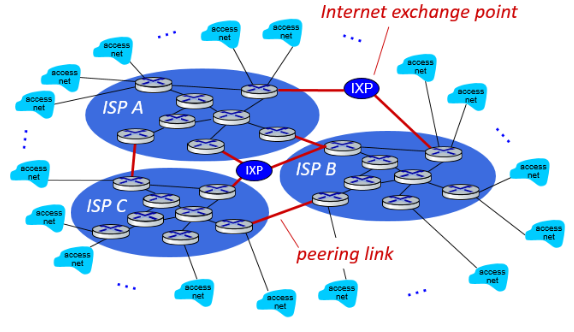
\includegraphics[width=0.5\linewidth]{State of the Art/KuroseISPs.png}
    \caption{Caption}
    \label{fig:enter-label}
\end{figure}

Governments leverage these nodes in the network topology to restrict user access to undesirable content.  Institutions will typically use a combination of legislative pressure, technological and economic means to snuff out content. ISPs and VPNs face significant and constant pressure from legal arms to expose user data and manipulate the content available to a user. In his research paper from 2003, Zittrain gives a solid overview of points of control. One issue he raises is the violation of the end-to-end principle. Simply, this refers to keeping the middle of the network simple and pushing complexity out towards the edge of the network to hosts. The presence of middleboxes and other devices could be impacting performance of the network. "The technical aspect of the end-to-end argument suggests a warning against blocking data transmissions at any point [other than endpoints]." \cite{Zittrain_Internet_Points_of_Control} 

Although security considerations such as HTTPS and TLS can help protect users from threat actors, points of control are a physical reality to be contended with. As user packets traverse the network they are subject to inspection. In this way, points of control are a key consideration for all internet users. Zittrain concludes his research with a word of warning regarding points of control and their potential for abuse. He highlights the need for "a comprehensive framework where sovereigns’ actions to block material are thoroughly documented and open to challenge." \cite{Zittrain_Internet_Points_of_Control} 

\subsection{Legislative Pressure}
Governments can enforce censorship directly through ISPs, tech companies and social media platforms by creating new legislation or simply mandating content be removed. This is used to de-platform individuals and movements during periods of unrest. This is also done in app stores, shutting down entire platforms that are deemed problematic. More commonly, judiciary process is used in democratic states to block access to illegal sites. Blocking will then be implemented through DNS servers, ISPs, institutions, service providers or otherwise in accordance with court orders. 

VPN providers are subject to the scrutiny of the jurisdiction within which they operate. NordVPN, a very popular VPN provider based in Amserdam has said on record "We will comply with lawful requests as long as they are delivered according to all the laws and regulations." \cite{nordvpnPrivacy2024} This reflects the reality of VPN services as provided by corporations. VPNs in this sense can be described as a double edged sword. In most cases they are very helpful in protecting user anonymity and circumventing censorship. However, if legislative pressure is applied, corporations will have no choice but to comply with the demands of the government. This may be trivial and to be expected by most consumers of VPN services, however, security issues in open source and previously trusted projects like TOR represent a more grave concern. 

\subsection{MITM Attacks}
Kampourakis, Kambourakis, Chatzoglou, and Zaroliagis wrote an academic paper in 2022 arguing the effectiveness of MITM attacks against HTTPS in certain circumstance. They describe a MITM attack as follows. "A man-in-the-middle (MitM) attack enables threat actors to position themselves in a conversation between two parties. It can be used to eavesdrop on, or impersonate, either of the parties and may enable the perpetrator to steal personal information, including login credentials, payment card data and account details."\cite{MITMvHTTPS} A MITM attack simply involves a threat actor, or in this case a censor, placing themselves in the middle of a conversation, potentially at a point of control. Governments have been seen to pressure VPNs into routing traffic through designated MITM servers. Inevitably this allows for selective content manipulation, deep packet inspection and surveillance. MITM attacks are particularly concerning due to their covert and intrusive nature. 

RFC 2818, released in 2000, describes "how to use TLS to secure HTTP connections over the Internet," \cite{rfc2818}known as HTTPS. This was designed to mitigate the effects of MITM attacks. Recent research suggests deployments of HTTPS in most browsers is insecure, at least in certain circumstance. Kampourakis and his colleagues went on to say "some insidious variants of MitM against HTTPS remain quite realistic across all popular Internet browser types irrespective of the underlying platform." \cite{MITMvHTTPS} 
They mention how "both of the attack variations were successful against all the browser types and versions..." except the latest versions of Firefox that they tested.

\section{Network-Level Filtering}
The following section is based primarily on information from the source \textit{RFC 9505 A Survey of Worldwide Censorship Techniques} \cite{rfc9505}. Any other information sourced from elsewhere is identified as such.

\subsection{IP Blocking}
Originally implemented to stop email spam, Internet Protocol (IP) blocking is one of the most straightforward censorship techniques. Each device connected to the internet is assigned a unique numeric label called an IP Address, which serves as an identifier that allows data to travel across the internet to the correct destination. RFC 791 describes the function of the Internet Protocol, "to move datagrams through an interconnected set of networks." \cite{rfc791}

When a government or ISP wants to censor a specific website it can be implemented in either incoming or outgoing traffic. ISP controlled firewalls can be configured so that any outgoing or incoming requests to a selected IP address are dropped. ISPs can also adjust routing tables in their network to remove an IP address, making it unreachable for the user. In a 2009 report, Callanan and co. describe how "the server that contains the website could be blocked at the level of its IP address, preventing anyone using the filter from accessing that address." \cite{inthemis2025internet} IP blocking can either be implemented at a centralized level or at an ISP level. In Ireland, IP blocking is done at an ISP level to block certain illegal websites. The primary motivation for the Irish government in doing this is to crack down on piracy. A prime example discussed previously is the blocking of the Pirate Bay. \cite{piratebay_block2013}

\begin{figure}
    \centering
    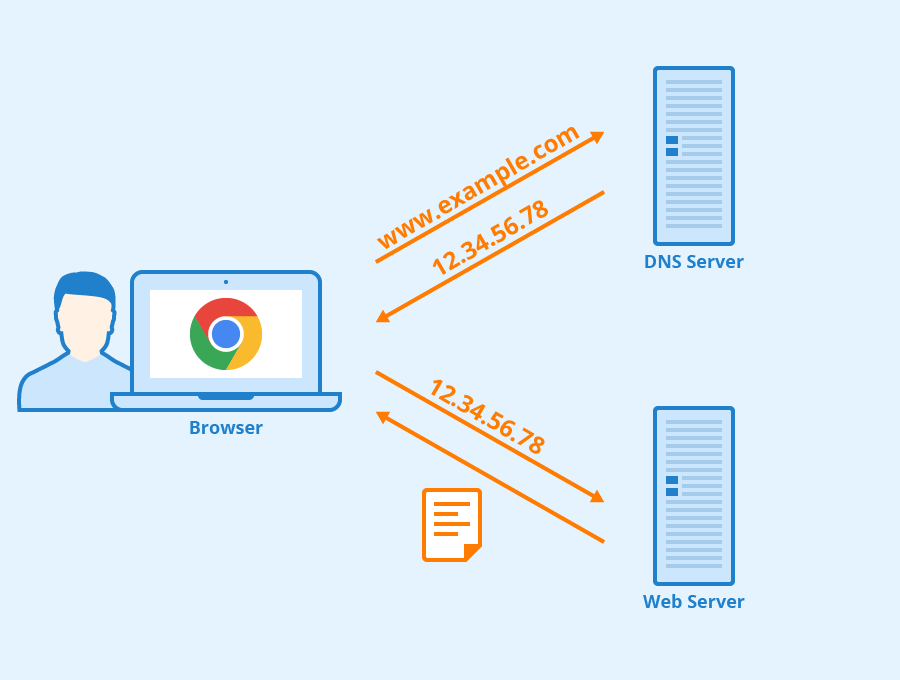
\includegraphics[width=0.5\linewidth]{State of the Art/DNS.png}
    \caption{DNS Requests and IP}
    \label{fig:enter-label}
\end{figure}


\subsection{DNS Interference}
DNS interference refers to the altering of responses from the DNS to block or filter access to certain content. This is usually done by either blocking the response, replying with an error message, or responding with an incorrect address. 
\textit{DNS Mangling} is a network-level technique of on-path interception where an incorrect IP address is returned in response to a DNS query to a censored destination. 
\textit{DNS Cache Poisoning \& Lying} is an off-path technique in which a censor intercepts and replaces the legitimate response from an authoritative DNS name server with a spoofed IP address. Instead of allowing the real IP address of a site to reach the user, the censor replies faster than the real server, and that spoofed IP gets cached (perhaps by numerous recursive resolvers). Subsequent requests will then be redirected to an incorrect IP, normally leading to a warning page or a meaningless domain. DNS lying on the other hand involves the censor mandating that the DNS server provide a particular response. Of all of the methods to tamper with DNS resolution this is the most aggressive. \cite{rfc9505}.

The above DNS interference methods require the censor to traverse a controlled DNS hierarchy for this mechanism to be effective. This mechanism can be circumvented by using a different publicly known DNS resolver that is not controlled by the censor. This mechanism can also lead to unintentional blocking in area's not controlled by the censor. For example, sometimes a user outside of the censor's region will be directed through DNS servers controlled by the censor, causing the request to fail. 

\subsection{Network Blackouts}
A very straightforward, holistic, and blunt form of censorship is network blackouts. This method involves a large governing body of an area or region completely shutting off Internet access for all content. This method is becoming more and more common across areas in the Middle East and Asia. According to a report from \textit{Access Now}, there were a total of 296 different internet shutdowns across 54 countries. \cite{accessnowBlackoutReport2023} This is a 35\% increase from the previous high in 2022 \cite{internetblackouts}. This form of censorship is very extreme and is often implemented in times of conflict, protest and democratic instability. 


\section{Keyword Filtering \& Deep Packet Inspection}
So far, methods of internet censorship have revolved around blocking a publishers address. However censors can examine the contents within packets to make decisions regarding their accessibility. This refers to the concept of application layer filtering; monitoring a communication channel and detecting offensive keywords. This is seen in more cultivated censorship models that strive to censor topic 'x'. 

\textit{Keyword Filtering} This approach involves scanning the contents of web requests for specific sensitive words or phrases. Upon encountering a request that contains a blacklisted keyword, the censor can disrupt the communication by, for example, sending TCP reset packets to both sides. This is a simple approach that is easily implemented. Pattil, in a 2014 paper, described this process saying "any packet that is passed across the network is scanned against a list of sensitive keywords and if present it forces the connection to terminate." \cite{uta-cse-1227} Circumventing keyword filtering is not particularly difficult. Coy publishers will employ deliberate misspelling or use of synonyms in place of sensitive keywords. 

A notorious example of keyword filtering in the real world is China's censorship of the 1989 Tiananmen Square protests. The Chinese government has been dedicated to removing this from the memory of its citizens, particularly the younger generation. \cite{nsarchive2001tiananmen} Louisa Lim, while researching this topic in 2014, polled Chinese students at four Beijing campuses and found that "out of 100 students, only 15 could identify the [Tank Man] picture." \cite{lim2014amnesia} In December of last year it surfaced that Tokyo University had embedded a keyword relating to the incident into one of its online applications. In an apparent attempt to prevent the page from loading in mainland China and stop Chinese students from applying, the university weaponised the Great Chinese Firewall. This is a prime example of the limitations of keyword filtering. \cite{unseenjapan2023tiananmen}

\textit{Deep Packet Inspection} DPI involves looking into payloads and data within packets, beyond its header. It is a sophisticated technique usually performed as part of a firewall defense and involves making real time decisions about the nature of each packet. DPI functions at the application level and can be used to identify both the sender and recipient of the packet by examining its payload. Compared to regular packet inspection which is only concerned with basic header information, it is considerably more costly. 

Deep packet inspection is used in specific cases where a higher level of audit is required. This includes packets carrying malware, content that has been blocked and intrusion efforts. DPI is usually performed by network middle boxes, devices that lie between end points. One of the these middle boxes is BlindBox, a system that accommodates DPI while preserving privacy and encryption. The creators of this system highlight the potential risks to user privacy with other black boxes. "To enable middlebox processing, some currently deployed middlebox systems support HTTPS in
an insecure way: they mount a man-in-the-middle attack on SSL and decrypt the traffic at the middlebox." \cite{sherry2015blindbox}

Though its deployment is limited, DPI represents a significant risk to user privacy. Not all middle box providers offer the protections and guarantees that BlindBox offer. Forecasts for the market show a troubling trend, with no guarantees of user privacy. "Global deep packet inspection (DPI) market size was anticipated to be worth USD 10.63 billion in 2024 and is expected to reach USD 79.26 billion by 2033 at a CAGR of 25\% during the forecast period." \cite{DPIMarketInfo}


\chapter{Circumvention Tools}
\section{Circumvention Tools}
Users who care about privacy and anonymity have options to increase their operational security and avoid censorship. Some of the most noteworthy tools are briefly explained below. It is worth mentioning that accessing these tools can be difficult for certain individuals. ProtonVPN discusses some of the countries that have outlawed VPN usage. \cite{protonvpn_vpn_legality_2} Some notable examples include Cuba, China, Vietnam and Egypt. This is a common theme; an arms race between oppressive regimes interested in censorship and circumvention and privacy based tools.

\textbf{Encryption}
Encryption is the fundamental security element driving communication over the internet. Bhanot describes encryption as "the process of converting normal data or plaintext to something incomprehensible or cipher-text by applying mathematical transformations or formulae." \cite{bhanot2015review} The importance of cryptography in security cannot be overstated. "Today, end-to-end encryption is the standard by which almost if not all communication over the internet occur. Examples of messaging platforms that offer this as standard include Telegram, Whatsapp and Facebook Messenger. CloudFlare states that end-to-end encryption "gives people total control over who can read their messages, enabling them to keep their messages private." \cite{cloudflare_e2ee} Encryption is the backbone of privacy online which allows users to leverage math to provide anonymity, at least in the best of cases. Zeadally, Das and Sklavos state the following about encryption "These techniques provide several security requirements, such as confidentiality, data integrity, entity authentication, message authentication, key management, non-repudiation, trustworthy data platforms, and digital signatures." \cite{ZEADALLY2021100075} It is clear from the research conducted that encryption benefits internet users. 

\textbf{Transport Layer Security}
Transport Layer Security (TLS) is an example of encryption being used to secure data transfer online. TLS replaced the deprecated Secure Socket Layers (SSL), and TLS 1.3 is the standard by which data is transferred over the internet. According to the Internet Society, "TLS is normally implemented on top of TCP in order to encrypt Application Layer protocols such as HTTP, FTP, SMTP and IMAP." \cite{internetsociety_tls_basics} TLS operation is described in detail in RFC 8446 \cite{rfc8446} \cite{cloudflare_tls_handshake}. Below is a figure that shows a TLS handshake.

\begin{figure}
  \centering
  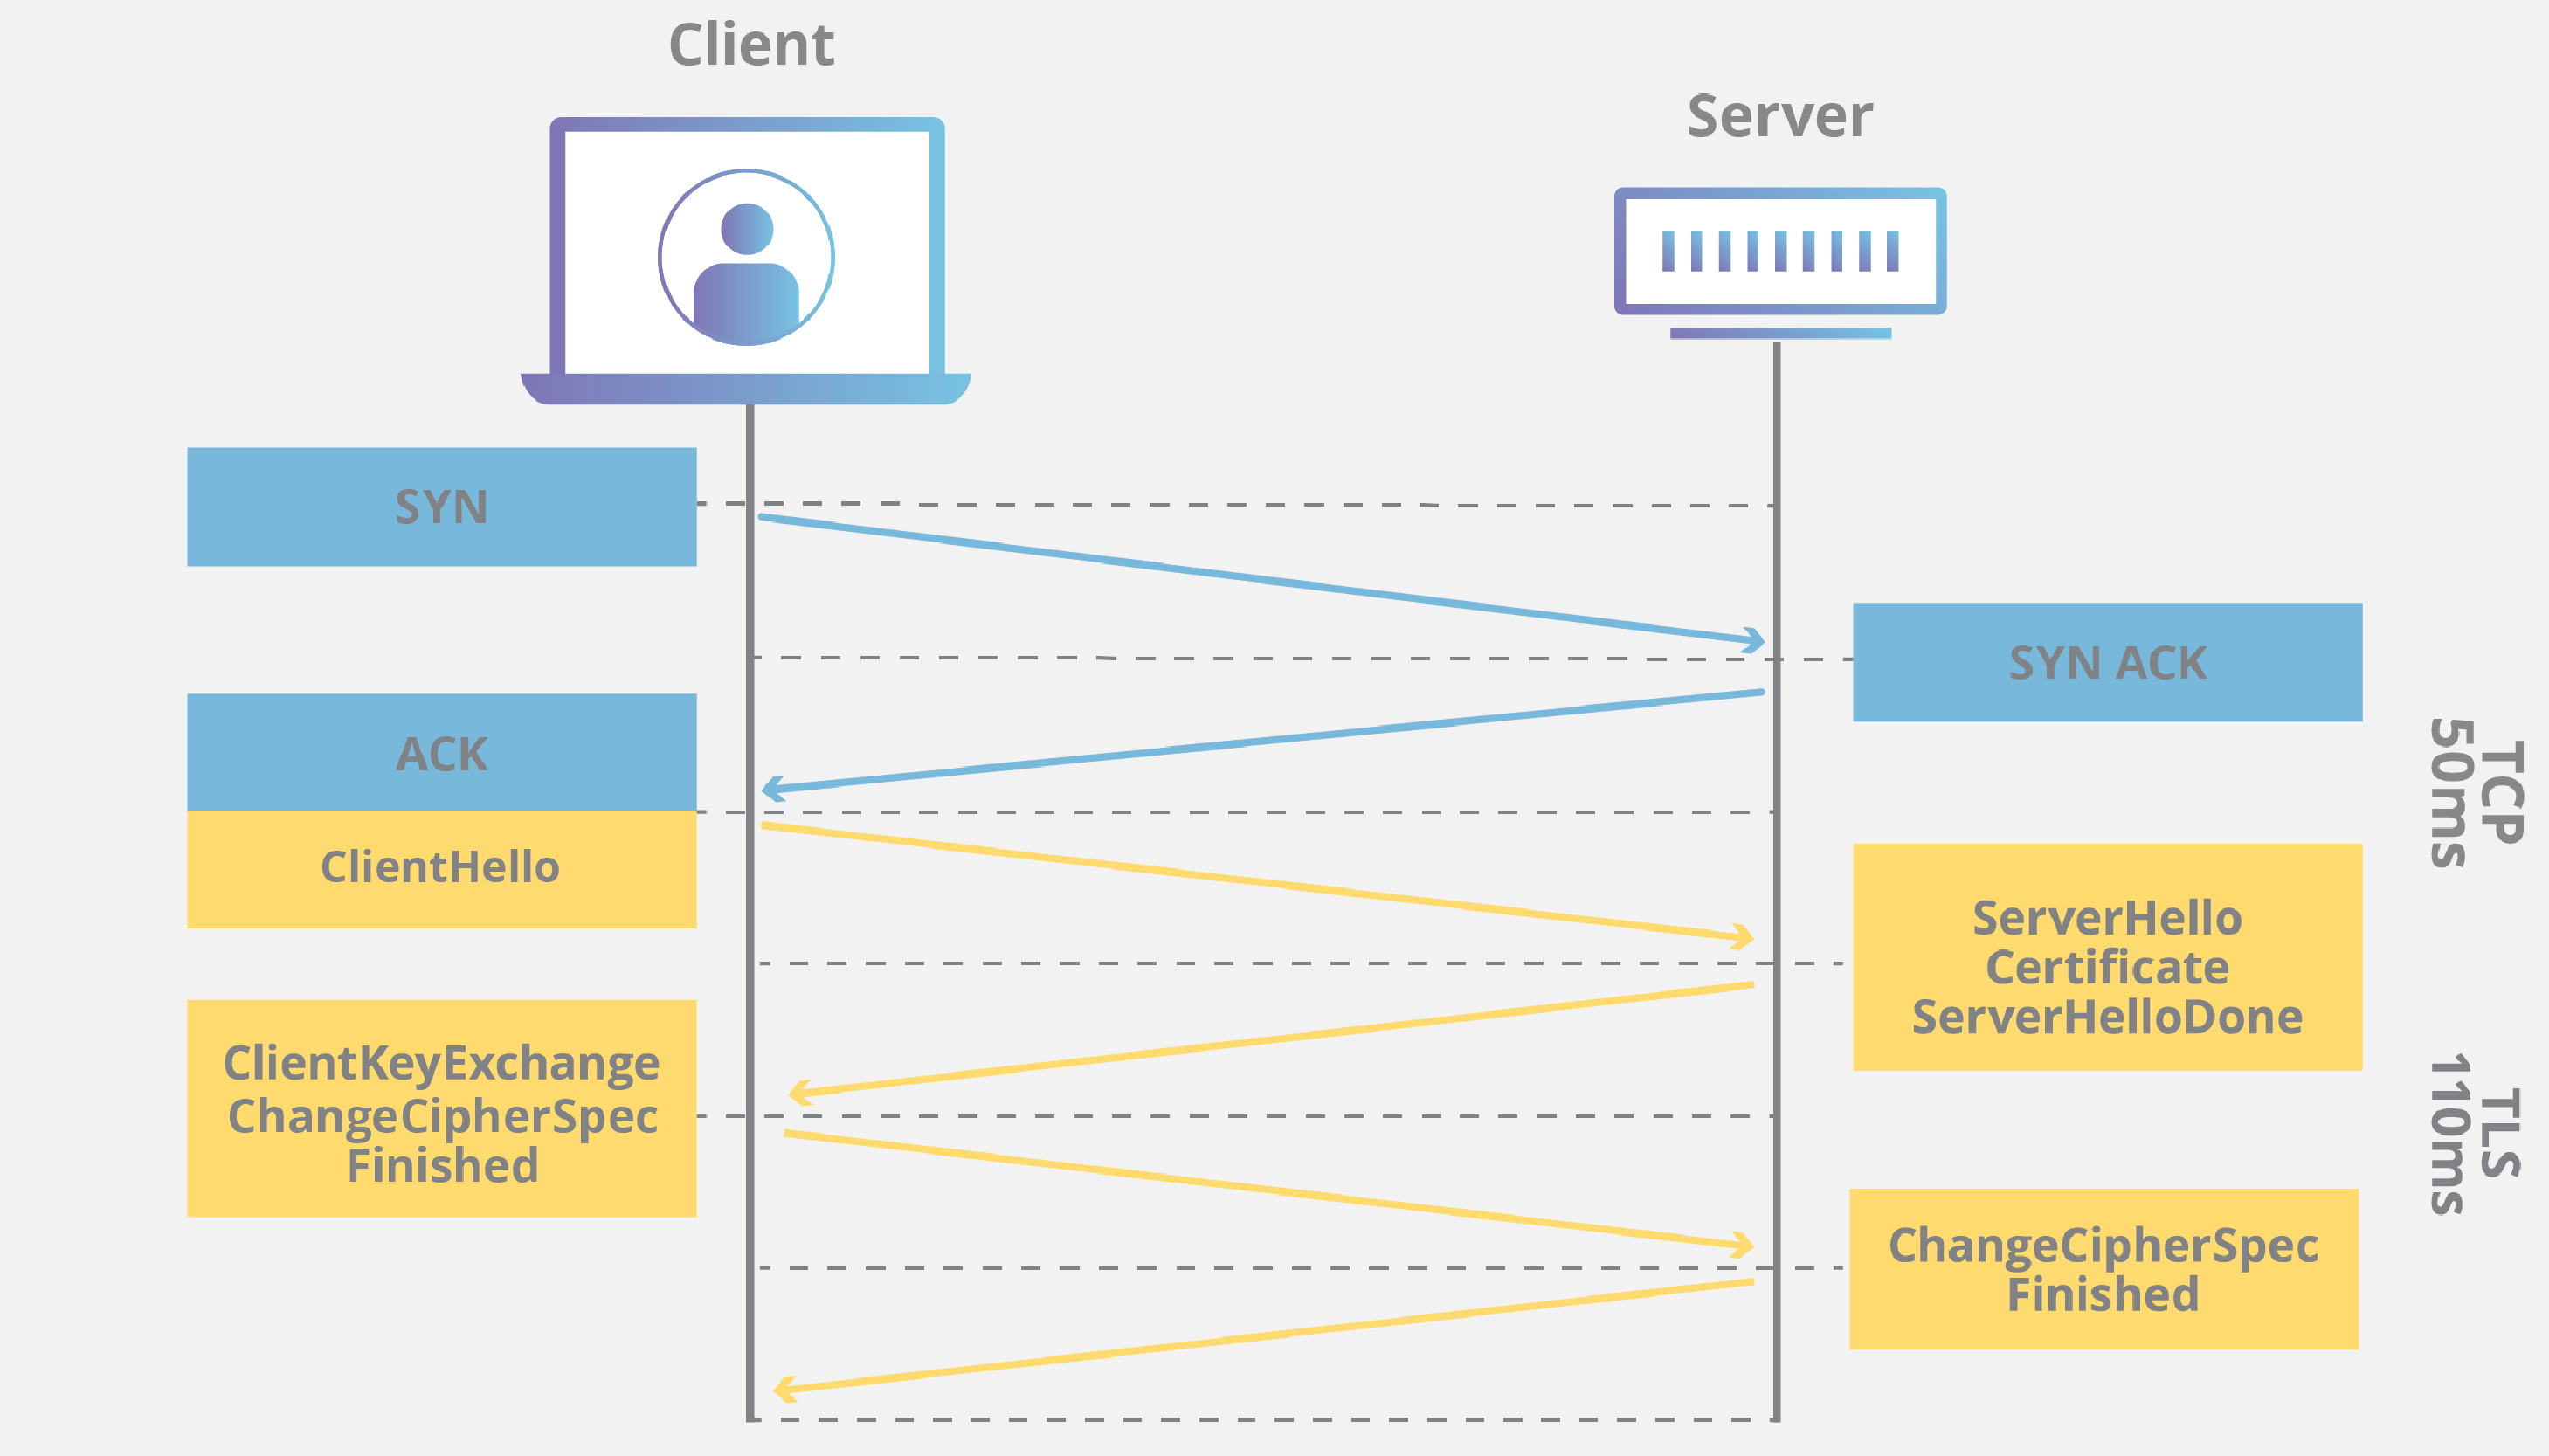
\includegraphics[width=\textwidth]{Circumvention Tools/TLS_Handshake.png}
  \caption{TLS Handshake, source cloudflare.com}
  \label{fig:your_label_here}
\end{figure}


INFO ABOUT TLS HANDSHAKE???

However, cryptography has not always had this virtuous reputation. The FBI lead what can only be described as a smear campaign against the technology in the early 2000s. In 1999, the director of the FBI, Louis Freeh, stated "encryption ultimately will devastate our ability to fight crime and prevent terrorism.” \cite{bitsbook_chapter5} Unsurprisingly, their stance has changed along with the growing necessity for encryption. Today, the FBI website states of encryption: "Law enforcement supports strong, responsibly managed encryption. This encryption should be designed to protect people’s privacy and also managed so U.S. tech companies can provide readable content in response to a lawful court order." \cite{fbi_lawful_access} The US government employs more methods than slander to defeat cryptography. The National Security Agency \cite{nsa_website} has a colourful reputation regarding its contributions to cryptographic standards. Dual\_EC\_DRBG was a cryptographic standard released by the NSA in 2007 and ratified by the National Institute of Standards and Technology (NIST). It was later found that this was insecure, having back door potential. CloudFlare defines a back door as "an intentional flaw in a cryptographic algorithm or implementation that allows an individual to bypass the security mechanism." \cite{cloudflare_nsa_backdoor} The discovery of this vulnerability is credited to Dan Shumow and Niels Ferguson. \cite{schneier_nsa_backdoor}



\textbf{Virtual Private Networks}
Virtual Private Networks (VPNs) are one of the most commonly used and important circumvention tools on the market. VPNs use tunnelling to encrypt packets at the lowest level, the OSI link layer. Microsoft developed Point-to-point Tunnelling Protocol (PPTP) which is now deprecated, having been shown to be insecure. \cite{microsoft_ptpt} More relevant examples of VPN protocols include IPsec \cite{rfc6071} and WireGuard \cite{wireguard_docs}. These protocols work by encapsulating packets and encrypting all of the information within. This provides secure data transfer over an insecure network. \cite{vpn_secure_connection2020} 

VPNs also allows users to effectively mask their IP address and change their apparent geo-location. This grants both privacy and circumvention potential; VPNs can be used to avoid geo - restrictions by routing traffic through more lenient countries. The role of VPNs in personal privacy and censorship circumvention cannot be overstated due to how commonplace the technology has become. According to SurfShark, a prominent provider, "over 1.6 billion people use VPNs." \cite{surfshark_vpn_users} Forbes states "Both the availability and usage of VPNs for personal use continue to rise," and this appears accurate. \cite{forbes_vpn_stats}

\textbf{The Onion Router (TOR)}
The Onion Router, originally developed by the US government, is an open-source network overlay that routes internet traffic through volunteer-operated relays. According to the founders, "Onion Routing is a distributed overlay network designed to anonymize TCP-based applications like web browsing, secure shell, and instant messaging." \cite{dingledine2004tor}

\begin{figure}
  \centering
  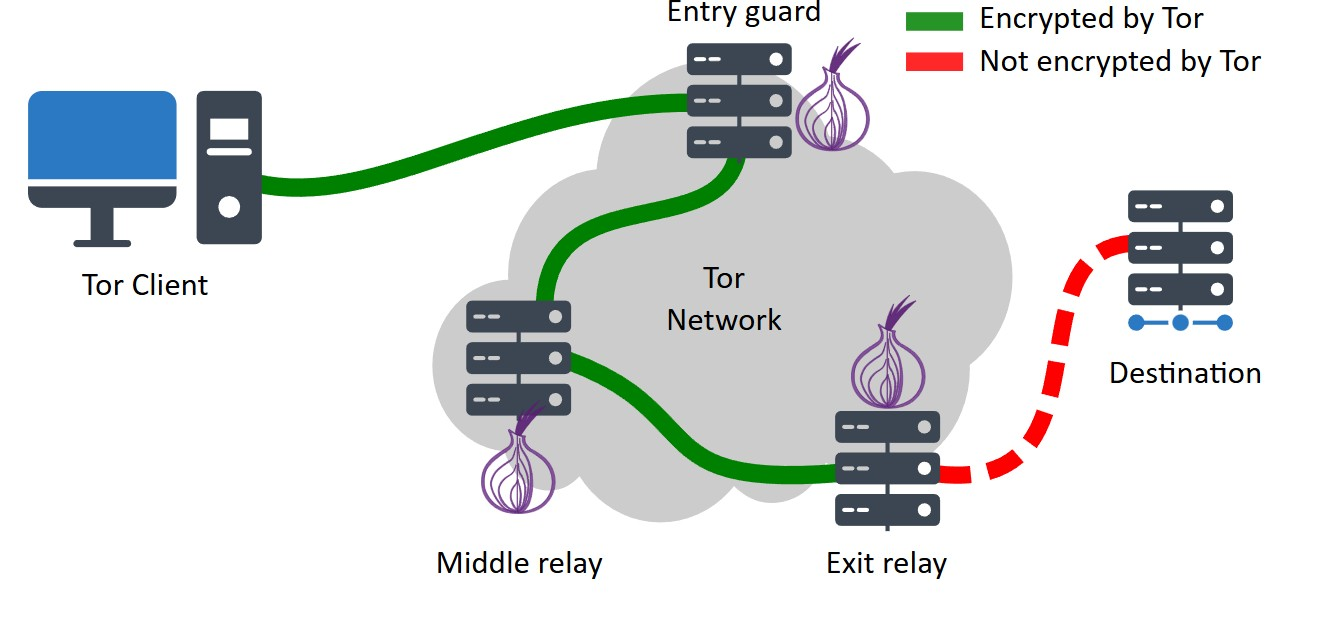
\includegraphics[width=\textwidth]{Circumvention Tools/How tor works.jpg}
  \caption{How TOR works}
  \label{fig:your_label_here}
\end{figure}

Requests travel through a relay passing three separate nodes. As a result, it is significantly more difficult to interpret the request’s origin and destination. Aside from granting privacy, Tor is also commonly used as a censorship circumvention method. Tor was believed to be secure for a long time but recent developments would suggest otherwise. \cite{tor_not_secure}

\textbf{TOR Bridges}
Previously, we have mentioned TOR relays and how three of them make up a circuit. The first hop over a relay is an important one; TOR bridges act as the first relay in certain circumstance. "Bridges are onion routers in the Tor Network whose IP addresses are not public." \cite{matic2017dissecting} Bridges act as a hidden and flexible way to access the TOR network. This allows individuals, (particulary in countries where TOR is heavily blocked), to bypass censorship, communicate securely and enhance privacy. For example, TOR bridges have been used to access TOR within China. \cite{dunna2018analyzing} \cite{cyberly_tor_blocked}


\textbf{Psiphon}
Psiphon is a "free and open-source Internet censorship circumvention tool that uses a combination of secure communication and obfuscation technologies." \cite{psiphon_guide} During the 2021 Cuban protests, the government shut down several social media sites. This lead to over 1 million protesters using Psiphon as a circumvention method. \cite{bloomberg_cubans_evade_internet} 

Typically, circumvention tools either divert web traffic so it avoids the machines that filter, or disguise the traffic as that that does not need to be filtered. Psiphon state on their website that "the Psiphon app has the ability to relay traffic through various communication protocols. It attempts to connect through different protocols until a connection is made." \cite{psiphon_guide} As previously mentioned, this technology has proved its value in combating internet censorship. 

\chapter{Methodology}
\label{chap:Methodology}

\section{Collecting Data: OONI}

\subsection{Background}
Released under the TOR project in 2012, the Open Observatory of Network Interference (OONI) is a non-profit open-source software project whose goal is to empower decentralized efforts to document internet censorship worldwide \cite{ooniAbout}. The OONI organization openly publishes measurements and provides a public archive of network interference across the globe. This has produced a database of more than 2.6 billion individual tests. \cite{OONIExplorer}

OONI data has been used extensively by third parties both for research and advocacy. Examples include the Freedom on the Net 2024 \cite{freedomhouse2024struggle} report, iMAP reports \cite{ooni2024imap} by Sinar, and Access Now’s annual \#KeepItOn 2023 Report. \cite{accessnow2023keepiton} \cite{ooni2024yearinreview} Based on these high profile endorsements and the wealth of data available, OONI is a perfect tool to measure internet censorship.

\subsection{OONI Probe}
Released in 2017, the OONI Probe is a mobile app and software designed to test internet censorship. Users can install and run this software, contributing to the growing dataset in the OONI database. OONI's mission is to \textit{“ensure a free and open internet by increasing transparency of internet censorship worldwide.”} While no user appears to have faced repercussions from using the OONI probe, this may lead to a false sense of security or incorrect assumptions about anonymity. As emphasized in OONI’s onboarding quiz, probe tests can be visible on the network.

The OONI Probe CLI v3.24.0 was used during testing as it is the most recent stable release. Its documentation can be found on GitHub \cite{oonicli2024}.

\subsection{Virtual Machine}
In order to gather ground truth, a virtual machine in Israel is used to run OONI command line interface locally. This machine is accessed via SSH. These technologies will be discussed further below. The chosen provider, \textit{interhost.co.il}, has a strong track record regarding data integrity and security; however, further scrutiny is necessary. \cite{interhost} 

These tools were audited for any security and privacy concerns and the results are below. Tools like CloudFlare's TCP reset dashboard \cite{cloudflare_policy_blog} gave further insight on instances of throttling, blocking or otherwise. In order to expand the web connectivity tests included with OONI, resources like Citizen Lab's sensitive domain list were included. \cite{citizenlab_testlists} 

\section{Ground Truth: Ireland \& Israel}
To gather ground truth in Ireland, the OONI probe Command Line Interface was installed and ran over a two week period. Since the CLI is not natively supported on Windows, a Unix-based operating system was flashed onto a Raspberry Pi 5, which served as a dedicated headless testing device. The device was accessed remotely via SSH, enabling the automation and management of tests. 

\begin{figure} [H]
    \centering
    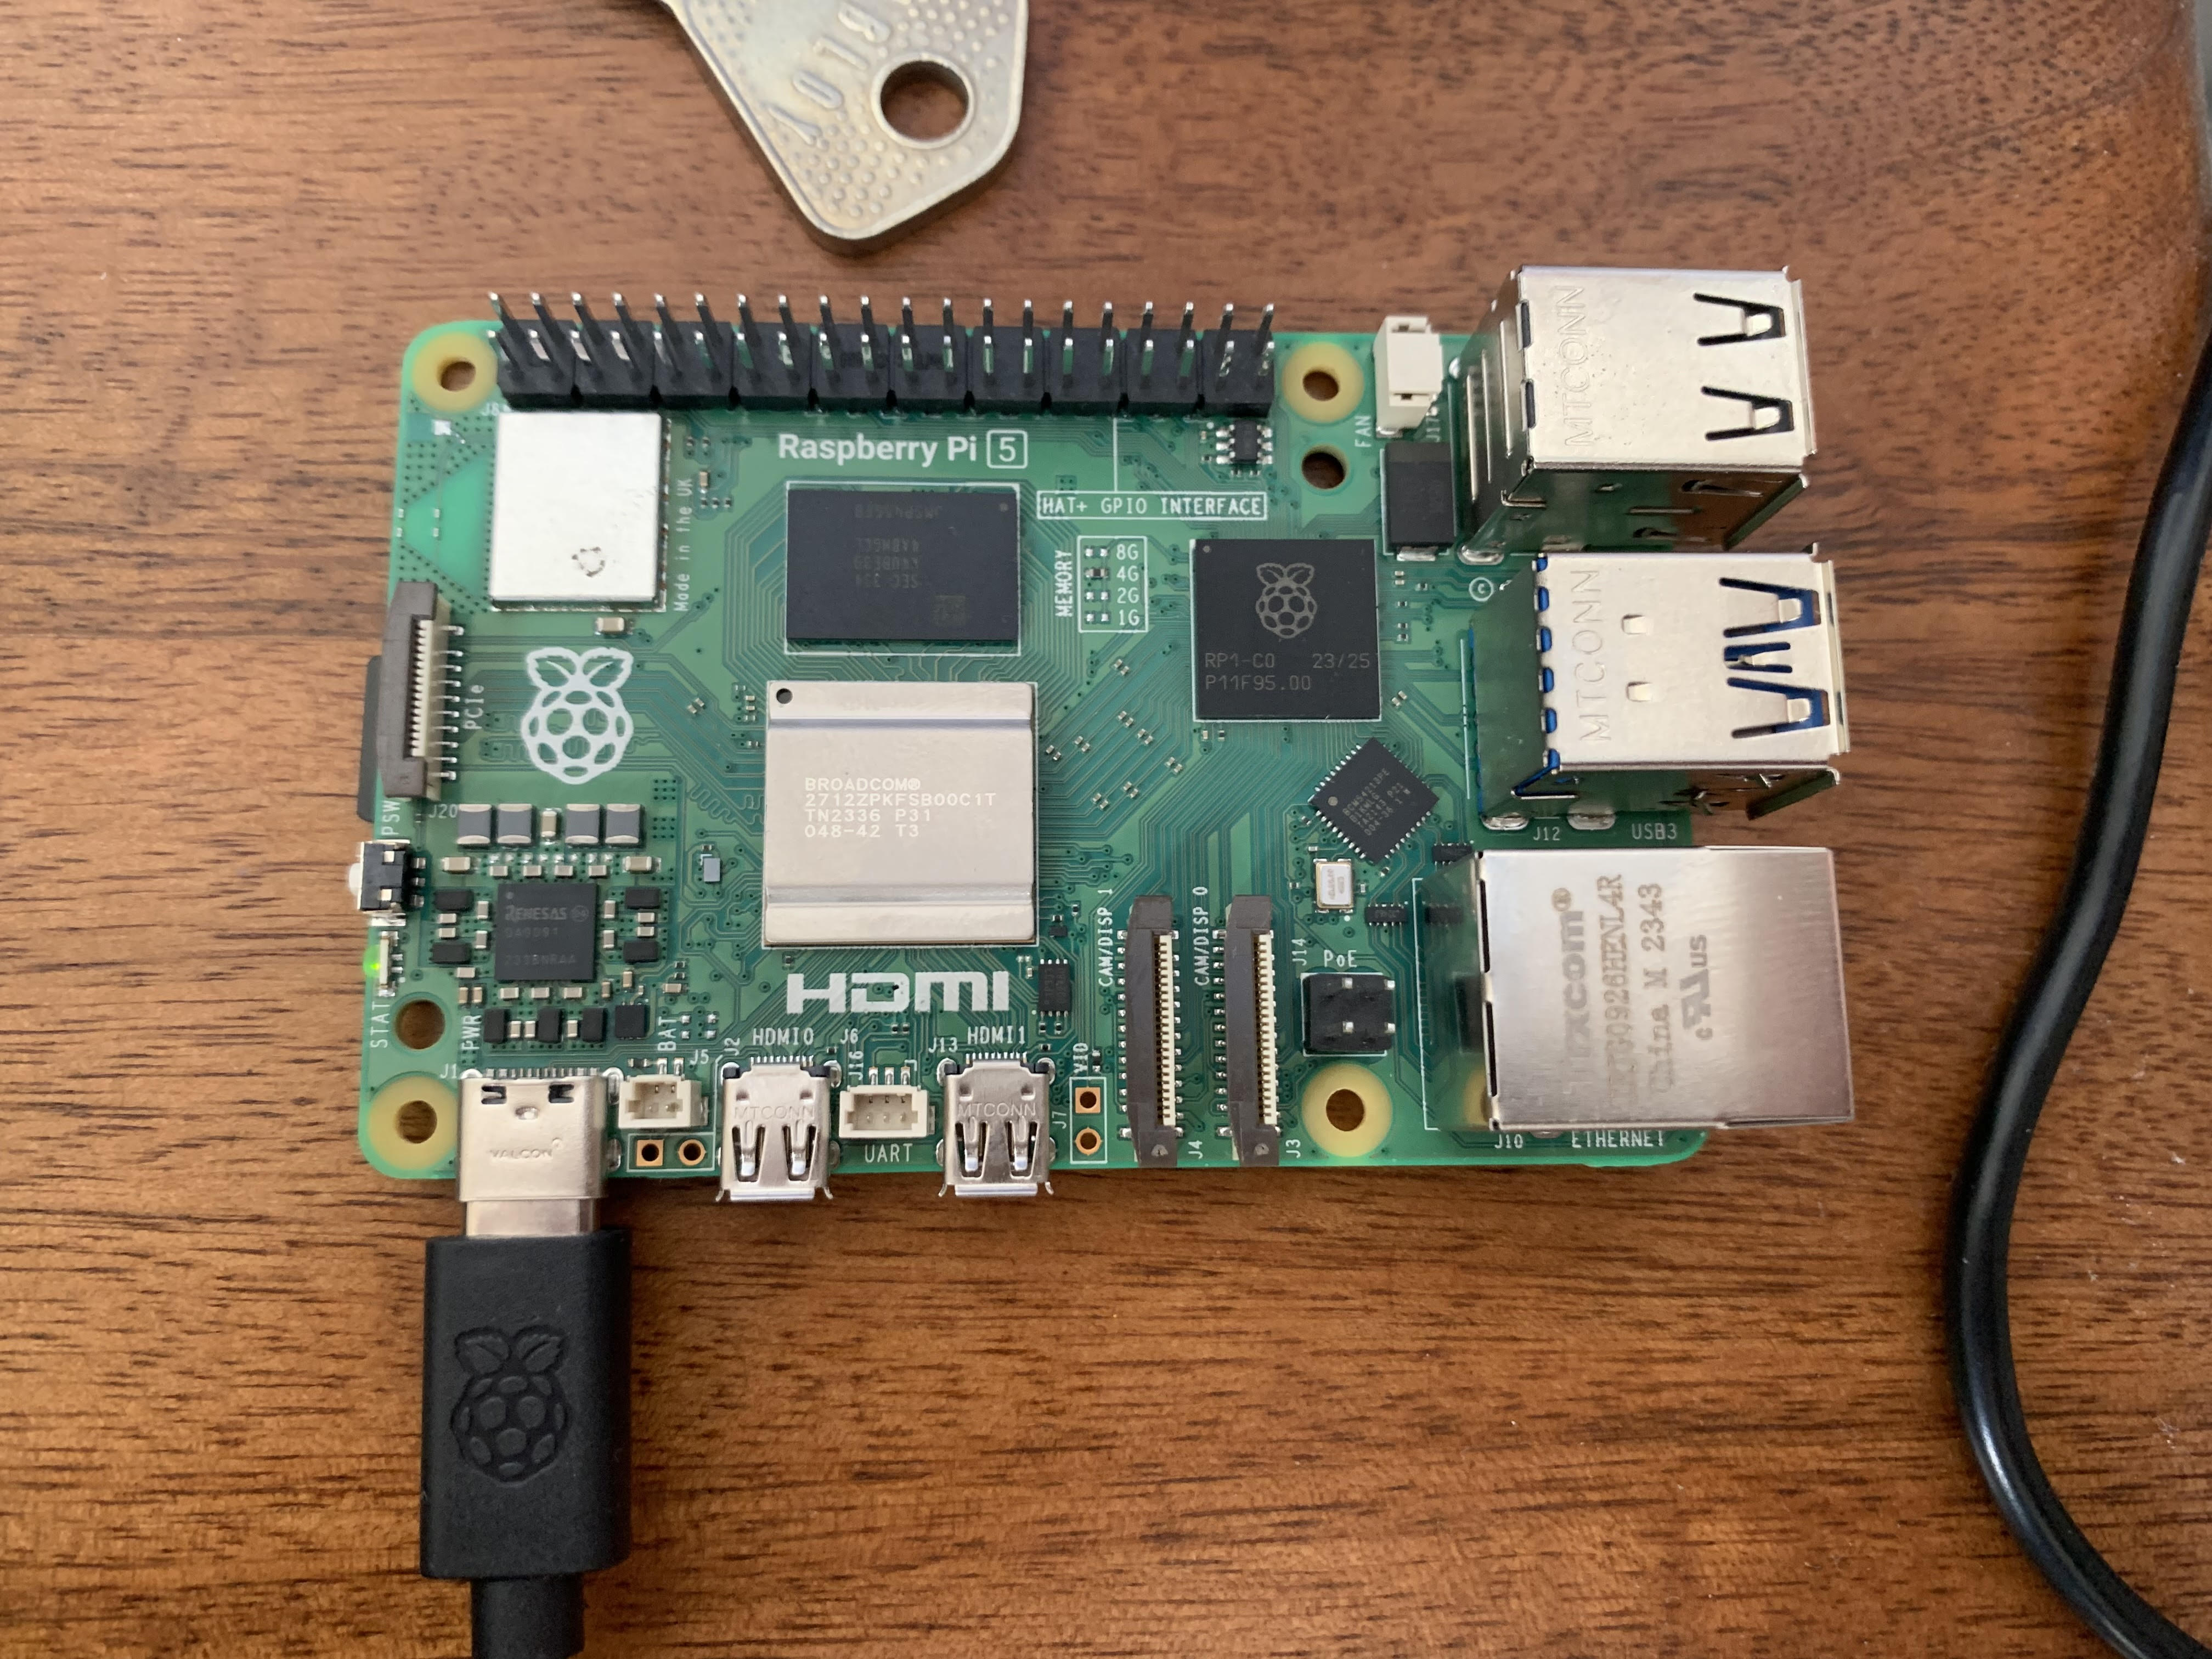
\includegraphics[width=0.5\linewidth]{RasPi5.jpg}
    \caption{Headless Raspberry Pi 5}
    \label{fig:enter-label}
\end{figure}

A similar process was used to remotely control the Israeli VM. This allowed for side-by-side running of tests and comparison of results. 

\begin{figure} [H]
    \centering
    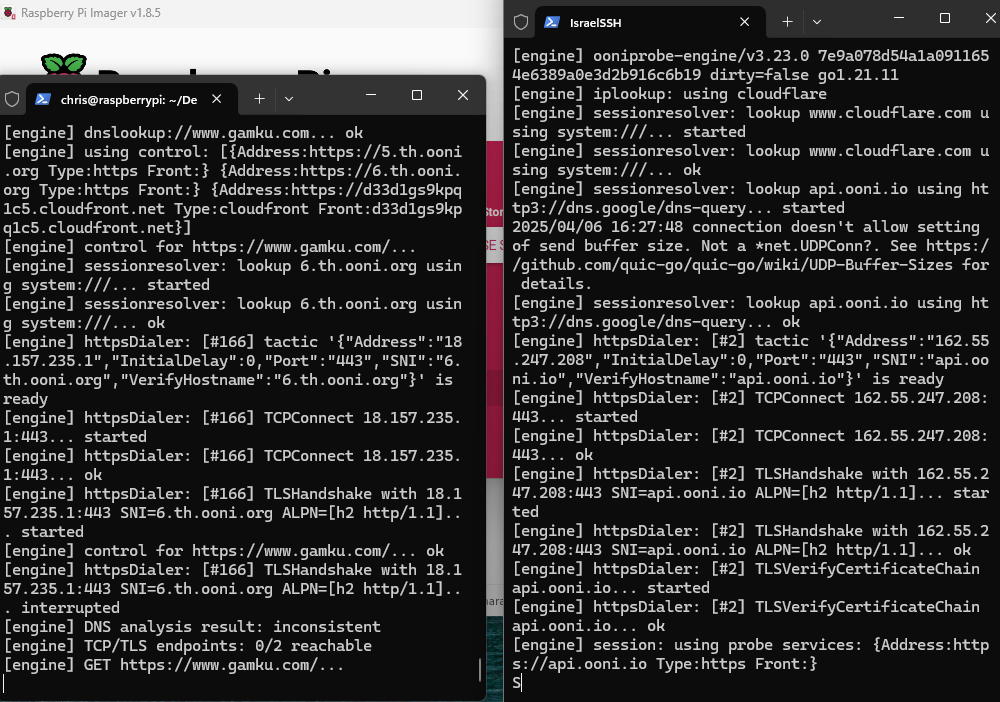
\includegraphics[width=0.5\linewidth]{RunningTestsSideBySideSSH.png}
    \caption{Running OONI tests over SSH}
    \label{fig:enter-label}
\end{figure}

\subsection{Description of OONI Tests}
\subsubsection{Web Connectivity Test}

The Web Connectivity test determines if, and how, access to a specific website may be blocked. To do this, OONI Probe performs several checks from the network where the test is run and compares the results with measurements collected from a control network where censorship is not expected. If the measurements differ significantly, censorship techniques are likely used on the local network. This test is designed to perform the four different actions: Resolver Identification, DNS Lookup, TCP Connect, HTTP GET Request.

The Web Connectivity test begins by identifying the DNS resolver in use on the network. It achieves this by sending DNS queries to special domains, which disclose the resolver’s IP address. Once the resolver is identified, the test performs DNS lookups to determine which IP addresses (and potentially other host names) are mapped to the tested domain. After collecting that information, the test attempts to establish a TCP session on port 80 or port 443, depending on whether the URL uses HTTP or HTTPS. Finally, once the TCP connection is successful, the test sends an HTTP GET request to the server hosting the website; under normal circumstances, the server will respond with the requested webpage content \cite{ooniConnectivityTest}.

\subsubsection{Circumvention Test}

The circumvention test is used to check weather Psiphon, Tor, or RiseupVPN are blocked on a given network. These are tools used to circumvent censorship by utilizing VPN, SSH, and HTTP proxy technologies. 

The Psiphon VPN serves as a tunnel that enables you to circumvent censorship by connected you to an uncensored portion of the internet \cite{ooniPsiphonTest}. The Psiphon test first uses Psiphon’s own code to establish a Psiphon tunnel. After the tunnel is created, the test attempts to load a webpage to see if Psiphon actually works for accessing the internet. If the tunnel is successfully set up and the webpage loads, Psiphon is functioning on the tested network and can bypass censorship. If the tunnel is established but the webpage does not load, Psiphon is blocked in some way, preventing access to online resources. Finally, if the test cannot even create the Psiphon tunnel, it indicates that Psiphon is completely blocked on that network \cite{PsiphonTestGitHub}.

The Tor Test \cite{TorTestABOUTOONI} automatically checks whether Tor is accessible in a given network by examining the reachability of core components such as Tor directory authorities, OR ports, and obfs4 bridges. It first attempts to retrieve the Tor consensus from directory authorities, then tries to connect to OR ports (including those of directory authorities) via a TLS handshake, and finally tests obfs4 bridges through an obfuscated handshake. If all of these steps succeed, Tor is likely usable in the tested network (unless it is blocked in ways not covered by the test). If any step fails, Tor may be blocked and therefore unavailable on that network \cite{TorTestGitHub}.

The RiseUpVPN test evaluates if the bootstrap servers used during the self-configuration of the VPN clients can be reached. The test also checks if RiseupVPN’s gateways can be reached on different ports and transports \cite{RiseUpVPNTest}. This test was contributed by the LEAP collective \cite{leapLEAPEncryption}.

\subsubsection{Instant Messaging Test}

The Instant Messaging test is used to check weather WhatsApp, Facebook Messenger, Telegram, and Signal are blocked on a given network.

The Whatsapp test attempts to determine is there is any interference or blockage of it's App or Web Interface. To to this, the OONI probe attempts to perform an HTTP GET request TCP Connection, and DNS lookup to WhatsApp's enpoints. These include the endpoints used by the WhatsApp mobile app, the registration service, and the web interface \cite{ooniWhatsAppTest}. To conduct these tests, the OONI probe attempts to open TCP sockets towards WhatsApp endpoints on Ports 443 and 5222. If these connections fail or are rejected, it is seen as an indicator of blockage at the TCP level. The probe then verifies if the DNS resolution returned a valid IP address that is registered to WhatsApp. If the resolved IP address does not belong to WhatsApp, it can indicate DNS level blocking or tampering. And to check if the WhatsApp registration service is working correctly, an HTTP GET request is sent to the URL \url{https://v.whatsapp.net/v2/register}. The request is considered successful if there is no DNS, TCP connect, TLS (Transport Layer Security), or I/O error \cite{WhatsAppTestGitHub}. 

The Facebook Messenger Test is used to examine the reachability of the service within a tested network. The OONI probe begins by attempting to perform a TCP connect and DNS lookup to facebook's endpoints \cite{ooniFacebookMessenger}. The test verifies if Facebook Messenger endpoints resolve to consistently known IPs and if it's possible to establish TCP connections to them on port 443. For each endpoint tested, an A lookup for the domain name is performed and it is considered consistent if the IP is inside of a netblock linked to the \textit{Facebook Authonomous System Number} (AS32934) \cite{FacebookTestGitHub}.

The Telegram Test is used to examine the reachability of Telegram's app and web version within a tested network. The telegram access points (DCs) are those used by the desktop client, and they have six unique IP addresses. The test establishes a TCP connection to all of the access point IP addresses and attempts to send a POST HTTP request to each of them. If all TCP connections on ports 80 and 443 fail, Telegram is considered to be blocked at the TCP level. Otherwise, Telegram is considered to be working as intended \cite{TelegramTestGitHub}. 

The Signal Test is used to measure the reachability of the Signal messaging app within a tested network. The test checks if it is possible to establish a TLS connection and send an HTTP GET request to the Signal server endpoints \cite{ooniSignalTest}. A DNS query to \url{uptime.signal.org} is also performed to check if the backend servers are down \cite{SignalTestGitHub}. 

\subsubsection{Middlebox Test}

A Middlebox is a computer networking device that transforms, filters, and manipulates traffic for purposes other than packet forwarding. These include network address translators, load balancers, and deep packet inspection (DPI) devices. The presence of Middleboxes can lead to evidence of censorship and/or traffic manipulation, but it can also be indicative of a less malicious intent, such as network caching.

The OONI Middlebox test consists of two main operations: HTTP Header Field Manipulation and HTTP Invalid Request Line. The HTTP header field manipulation test emulates an HTTP request towards a server, but sends HTTP headers that have variations in capitalization. These requests are sent to a backend control server which send back any data it receives, and if these requests return exactly as we sent them, it is assumed there is no middlebox present. If the alterations of the headers come back normalized, it can be assumed that there was packet manipulation of some kind, leading to the confirmation of presence of Middleboxes It is worthy to note that false negatives can happen in this test, as some ISPs use highly sophisticated software that can disguise the presence of Middleboxes \cite{ooniHTTPHeader}.  

The HTTP Invalid request line test sends an invalid HTTP request to an echo service listening on the standard HTTP port, rather than a valid one. If the request is returned to the user exactly as it was sent, it can be concluded that there is no evidence of the presence of a Middlebox. However, it is possible that this invalid request can be intercepted by a Middlebox that triggers an error that is sent back to the probe. This is evidence that there is a Middlebox present in the network. It is worthy to note that false negatives are possible as some ISPs use highly sophisticated software that is designed not to trigger such errors \cite{ooniHTTPInvalid}. 

\subsection{Data Collection and Transparency}
All results from OONI Probe tests are automatically sent to OONI's servers and published on the OONI explorer. This transparency ensures that anyone can explore the measurements for themselves. OONI aggregates measurements by country, time, and type of test. It highlights "confirmed" cases of blocking when there is strong enough certainty in the test result, but it also publishes anomalies that might be considered false positives. 

The OONI team also work to release comparative analysis and real-time alerts for significant internet censorship related events. This would include events such as a sudden surge in social media blockage, or a complete drop off of internet traffic in certain areas. The OONI Mesaurement Aggregation Toolkit (MAT) can be used to visualize these events and potentially identify emerging trends. 

\section{Privacy \& Security Concerns}
The following section contains information on privacy and security concerns associated with the completion of the dissertation. This was completed in conjuncture with an assignment given in the CSU44302 Security and Privacy module. 
In writing a dissertation, it is crucial to consider the potential impacts of the research. This document discusses the security and privacy concerns associated with researching internet censorship. Initially, theoretical vulnerabilities will be explored. Specific cases such as Israel and Ireland will then be analyzed. Finally, a practical perspective will examine realistic security and privacy concerns, along with relevant case studies.

\subsection{OONI Probe}
OONI's positive track record is emphasized by the claim: \textit{“To our knowledge, no OONI Probe user has ever faced consequences as a result of using our software.”} \cite{OONIRisks}. The success of OONI is critically dependent on users conducting tests without repercussions. However, OONI outlines several scenarios in which running their probe may be unwise. This includes users residing in countries with a history of prosecuting similar activities, surveillance concerns, or legal restrictions on accessing content. Users who fall into one or more of these categories should be wary of the potential risks. In this context, operating in Ireland with no reason to believe I am under surveillance, I am considered a low-risk user.

\subsection{SSH \& Virtual Machine}
A virtual machine (VM) emulates a computer system. It is a file (.img) that contains instructions to create a virtual environment, leveraging physical PC resources. The provider was chosen based on location availability, with Interhost offering a machine in Tel Aviv. The shared nature of resources introduces vulnerabilities. The number of users sharing the same hardware is unknown, so file-sharing precautions were taken. Storing sensitive information on this VM may be unwise for these reasons.

SSH is a cryptographic protocol that allows users to securely and remotely control a machine over an unsecured network. It employs a client-server model with public-private key pairs for encryption and password authentication. In this project, SSH was used to remotely control the VM in Tel Aviv. Upon generating key pairs, authentication was established, and the VM became accessible. Provided secure settings are maintained and the private key is never shared, SSH is a reliable and trustworthy protocol \cite{SSHManual}.

\subsection{Other Security and Privacy Considerations}
Personal safety risks in researching internet censorship must be addressed. My supervisor highlighted that selecting a comparison country required more than just finding a contrast. Publishing documents that critique government censorship has historically been risky \cite{JulianAssange, EdwardSnowden}. However, this research is relatively low-risk. Particularly compared to cases like Assange or Snowden. MIFTAH, an organization advocating open dialogue on the Israel-Palestine conflict, reported 310 press freedom violations from 2000-2003 \cite{MIFTAHReport2003}. Although Israel has a history of reprisals, these incidents were tied to conflict zones such as Gaza. This research is not of a whistleblowing nature, reducing potential risks.

Researching Israeli state-sponsored internet censorship inevitably intersects with ongoing conflicts. The thesis remains unbiased and non-political. Historical events are included only to provide accurate context for internet censorship analysis. While Israel’s military has strong ties to information control \cite{IsraelCensorship}, it is crucial that internet censorship is examined from an empirical lense.

The security and privacy considerations for this project required assessing all tools used. OONI’s privacy and security protocols appear robust. Its strong track record reinforces this confidence. SSH, as a long-established protocol, remains secure when best practices are followed. Potential consequences of researching this area are more extensive than initially anticipated. However, given my threat model, adverse effects are unlikely. Best practices will continue to be followed to ensure nonpartisan, data-driven research.
\chapter{Results}
\section{Overview}
Tests were conducted over a two week period between 31/03/25 and 13/04/25. Seven days worth of tests were exported from both machines for comparison and analysis. The results are discussed below, with pertinent tables included in the Appendix section. In comparison, the OONI database that is publicly available was analysed for the dates 13/03/25 to 13/04/25. 

It is important to recognize that, particularly in the case of Israel, different individuals may experience censorship of the Internet to varying degrees. The research focuses on replicating the experience of the average Israeli living in Tel Aviv. Having previously discussed the Gaza Strip, it is clear that the user experience varies greatly between the two areas. Further research may look at comparing Internet censorship experienced internally in Israel, but that is outside the scope of this work.

In the following section, the relevant context regarding the network conditions while gathering ground truth will be discussed. Having previously highlighted the varying levels at which internet censorship can be conducted, let us now define the specific network characteristics under which the OONI probe was run for both countries.

\subsection{Network Environment Context: Ireland}
As mentioned, the OONI CLI probe is running on a Raspberry Pi 5 connected to a home residential network over WiFi. The provider is Virgin Media (AS12388), registered under Liberty Global B.V. ISP (AS6830). 

Details regarding the operating system flashed to the Raspberry Pi and packages required for this are illustrated below in the 'Guide to Replicating Results.' 

\subsection{Network Environment Context: Israel}
Ground truth gathering in Israel was done using a virtual machine as described in the section on methodology. The virtual machine is operates within a data center hosted by O.M.C. COMPUTERS \& COMMUNICATIONS LTD (AS44709), downstream of its owner Kamatera Inc. (AS36007). This differs from the residential network that is being tested in Ireland.


\section{Website Connectivity Tests}


\subsection{Ground Truth via SSH}
\subsection{Native Website Connectivity Tests}
This section details the results of the daily web connectivity tests performed using the command \textit{ooniprobe run}. 

\begin{table}[H]
\centering
\caption{Summary of Tested vs. Blocked Websites by Country (Native to OONI)}
\begin{tabular}{lcc}
\toprule
\textbf{Country} & \textbf{Tested} & \textbf{Blocked} \\
\midrule
Ireland & 1695 & 25 \\
Israel    & 1695 & 16 \\   
\bottomrule
\end{tabular}
\label{tab:blocked_summary}
\end{table}




\subsection{my-websites.txt}
This file contains the additional 170 website connectivity tests I wished to conduct. The list was compiled with Griff Steinman, and additional tests relating to Israel were added. The contents can be found within the Appendix section. Below is a summary of the results from the daily running of this additional web connectivity test suite.

\begin{table}[H]
\centering
\caption{Summary of Blocked vs. Unblocked Websites by Country (my-websites)}
\begin{tabular}{lcc}
\toprule
\textbf{Country} & \textbf{Unblocked} & \textbf{Blocked} \\
\midrule
Ireland & 151 & 19 \\
Israel    & 155 & 15 \\   
\bottomrule
\end{tabular}
\label{tab:blocked_summary}
\end{table}

The following figure illustrates the blocking methods for the additional web connectivity tests. See Appendix section for a more detailed breakdown of positive results for each locale.

\begin{table}[H]
\centering
\caption{Distribution of Blocking Methods Detected in Ireland \&Israel}
\begin{tabular}{lcc}
\toprule
\textbf{Blocking Method} & \textbf{Ireland} & \textbf{Israel} \\
\midrule
TCP/IP         & 15 & 13 \\
DNS            & 1  & 1  \\
HTTP           & 1  & 1  \\
Error/Failure  & 3  & 0  \\
\bottomrule
\end{tabular}
\label{tab:blocking_methods_comparison}
\end{table}

\begin{table}[H]
\centering
\caption{Blocked Websites by Category and Country}
\begin{tabular}{lccc}
\toprule
\textbf{Category} & \textbf{Total Websites Tested} & \textbf{Ireland} & \textbf{Israel} \\
\midrule
Uncategorized                      & 34 & 4 & 4 \\
Piracy / Streaming / File Sharing  & 21 & 6 & 4 \\
News / Media                       & 34 & 1 & 0 \\
Adult Content                      & 21 & 0 & 0 \\
Creative / Educational / Misc      & 15 & 1 & 1 \\
General / National Services        & 19 & 1 & 1 \\
Streaming / Social Media           & 9  & 0 & 0 \\
Religious                          & 5  & 2 & 2 \\
VoIP / Communication               & 4  & 1 & 0 \\
Gambling                           & 2  & 1 & 1 \\
Email/Privacy Tools                & 3  & 1 & 0 \\
Adult / Alcohol                    & 2  & 1 & 1 \\
LGBTQ+                             & 1  & 1 & 1 \\
AI / Technology                    & 1  & 0 & 0 \\
\bottomrule
\end{tabular}
\label{tab:category_block}
\end{table}

\subsection{Investigating Aljazeera.com}
Upon initial testing of Aljazeera blocking in Israel, it was surprising to see no evidence of blocking. To investigate further it was decided that the content of the site should be examined and a variety of URLs belonging to it should be tested. Particular attention was given to articles that were critical of Israel.

The file sample\_aljazeeraurls.txt contains 100 URLs for articles hosted on https://aljazeera.com. Below are some helpful commands used to obtain the sitemap and extract URLs for testing. Wget was used to examine the contents of the web page, and the following was observed.

Despite preconceived notions, Aljazeera and its articles were not found to be blocked on AS44709. Reasons for this will be explored in the coming chapter.

\begin{figure} [H]
    \centering
    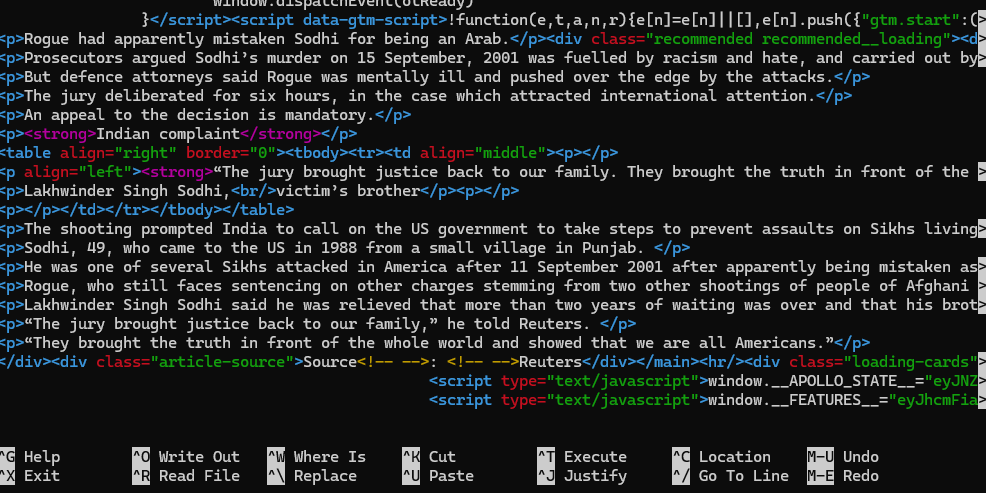
\includegraphics[width=1\linewidth]{wgetAljazeera.png}
    \caption{wget showing aljazeera.com content}
    \label{fig:enter-label}
\end{figure}


As seen above, I was able to see unblocked content from the site. Within Appendix, one can find a sample of articles being tested. 

\subsection{Public OONI Database}
In this section, the OONI database will be explored. As mentioned previously the period to be considered is 13/03/25 to 13/04/25. Below are screenshots of all web connectivity tests conducted in Ireland and Israel for these dates. 

\begin{figure} [H]
    \centering
    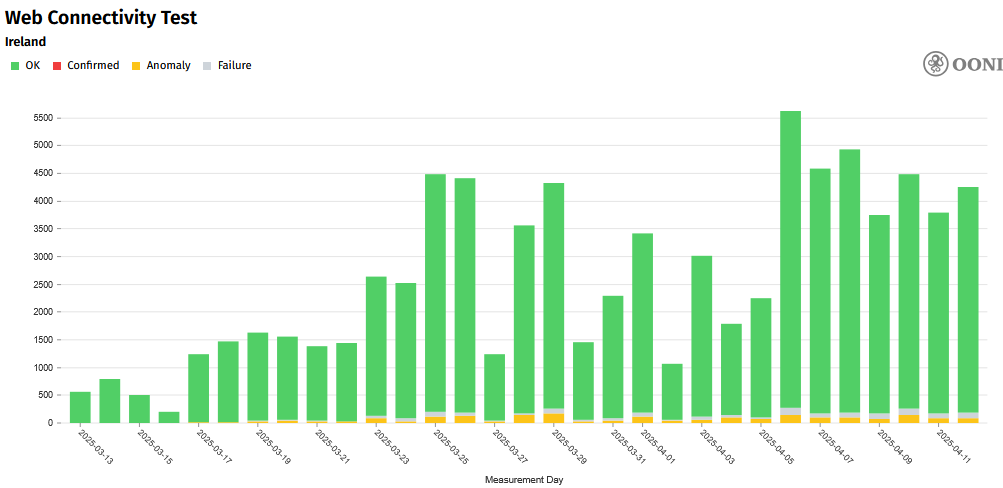
\includegraphics[width=1\linewidth]{IREWEBSOONIDB.png}
    \caption{Irish OONI Database Web connectivity tests 13/03-13/04}
    \label{fig:enter-label}
\end{figure}

\begin{figure} [H]
    \centering
    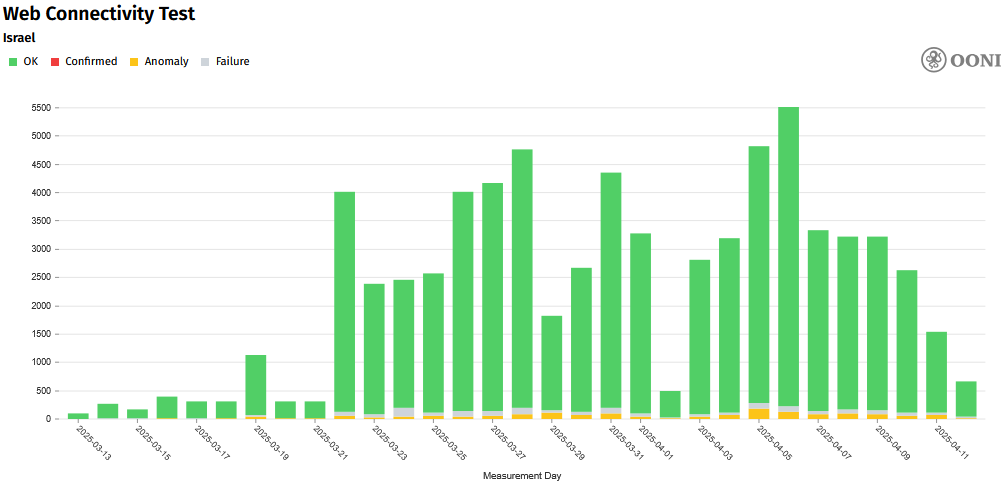
\includegraphics[width=1\linewidth]{ISRWEBSOONIDB.png}
    \caption{Israel OONI Database Web connectivity tests 13/03-13/04}
    \label{fig:enter-label}
\end{figure}

Further insight into this data can be seen through the proceeding table that documents a daily averages. 

\begin{table} [H]
\centering
\caption{Website Blocking based on Public OONI Data}
\begin{tabular}{lcc}
\toprule
\textbf{} & \textbf{Ireland} & \textbf{Israel} \\
% \midrule
Number of Websites Tested           & 2603 &  2299 \\
Number of Successful Connections    & 2491 & 2195 \\
Number of Anomalies                 & 67 & 53 \\
Number of Failures                  & 46 & 51 \\
\bottomrule
\end{tabular}
\label{tab:category_block}
\end{table}

By examining the publicly available data on Aljazeera and filtering based on ASN, an interesting picture emerges. There is clear evidence of large scale DNS tampering on certain ASNs, while others go unblocked. Prior to my testing using the VM in Tel Aviv, it was unknown whether O.M.C. COMPUTERS \& COMMUNICATIONS LTD (AS44709) was blocking this content. 

\begin{figure} [H]
    \centering
    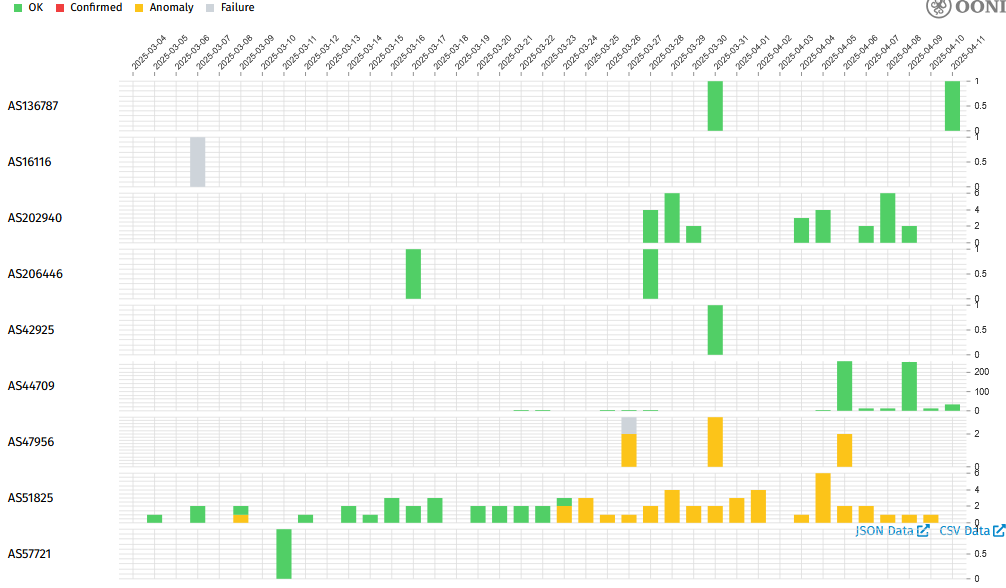
\includegraphics[width=1\linewidth]{ALJZRbyASN.png}
    \caption{OONI data (04/03/2025 - 11/04/2025) showing blocking of Alazeera.com grouped by ASN}
    \label{fig:enter-label}
\end{figure}



\section{Instant Messaging Tests}
By analysing the publicly available OONI data for both countries for the period of interest we can see little evidence of blocking of instant messaging platforms in either country.

\subsection{Public OONI Database: Ireland}
As seen in the below figures, there is little evidence to suggest network interference of instant messaging platforms in Ireland over the period considered.

\begin{figure} [H]
    \centering
    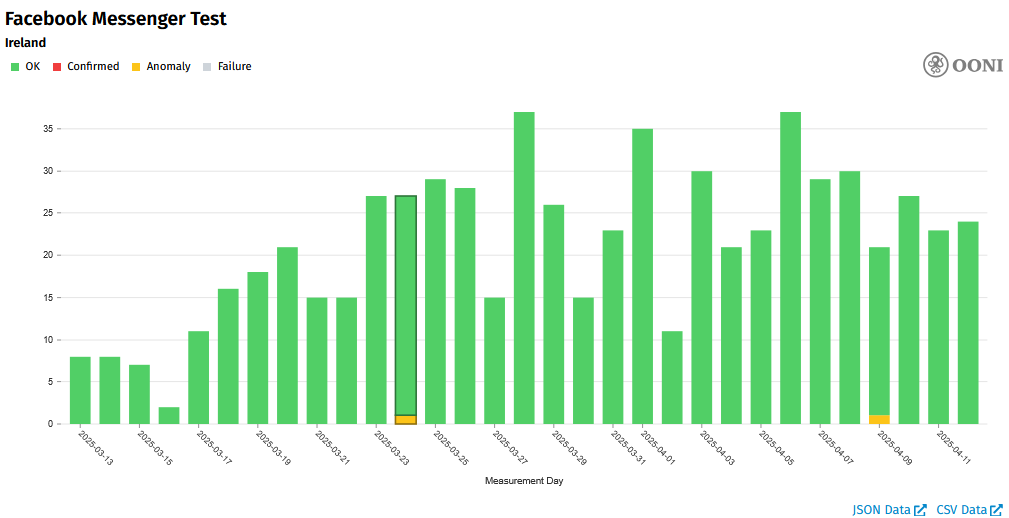
\includegraphics[width=0.5\linewidth]{IREOONIDBIMFB.png}
    \caption{Facebook Messenger test results for Ireland 13/03-13/04}
    \label{fig:enter-label}
\end{figure}

\begin{figure} [H]
    \centering
    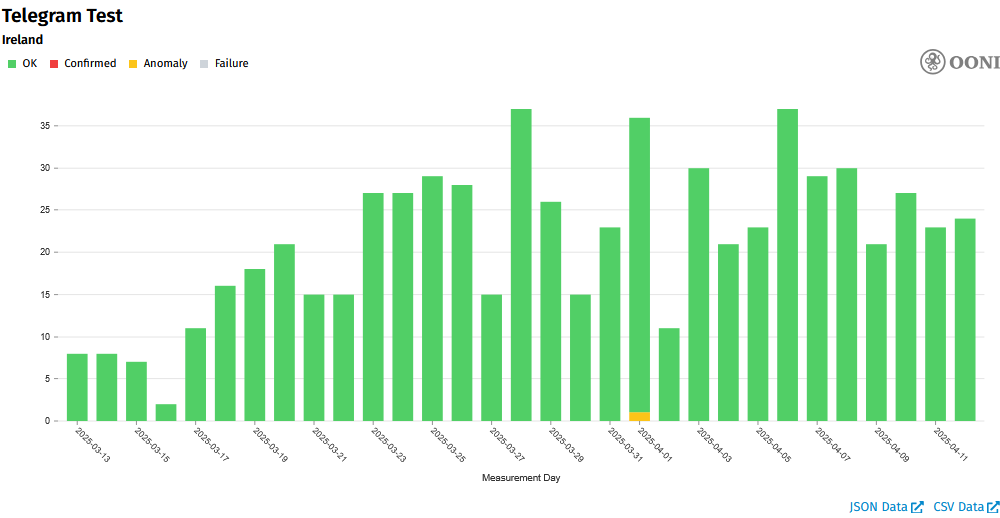
\includegraphics[width=0.5\linewidth]{IREOONIDBIMTL.png}
    \caption{Telegram test results for Ireland 13/03-13/04}
    \label{fig:enter-label}
\end{figure}

\begin{figure} [H]
    \centering
    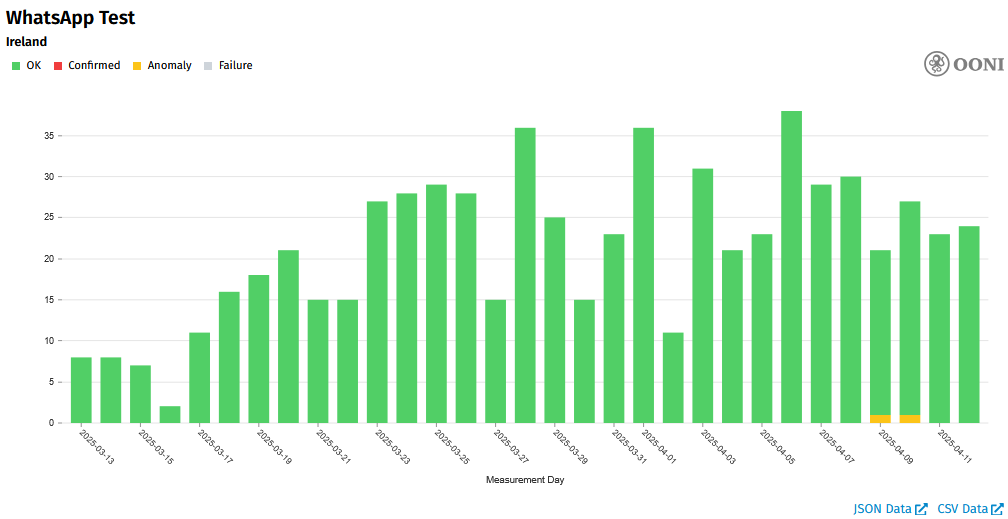
\includegraphics[width=0.5\linewidth]{IREOONIDBIMWHATS.png}
    \caption{WhatsApp test results for Ireland 13/03-13/04}
    \label{fig:enter-label}
\end{figure}

\begin{figure} [H]
    \centering
    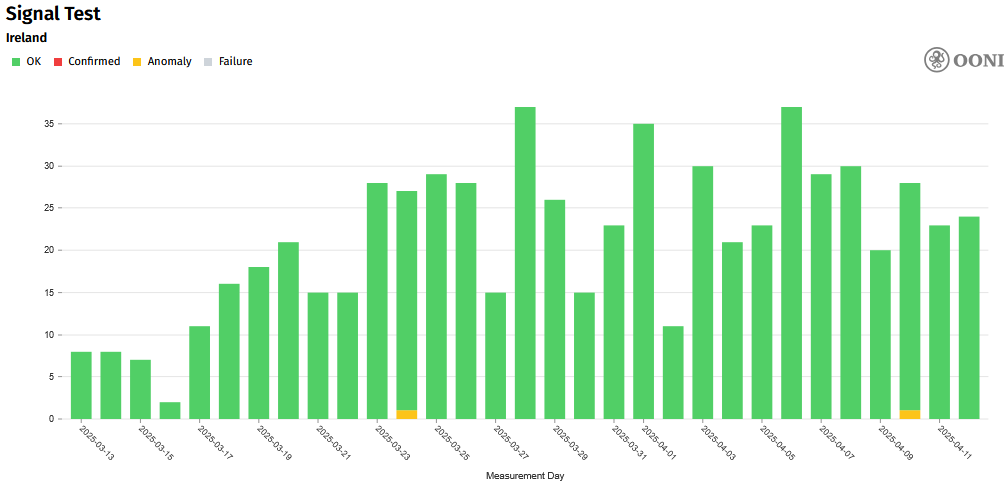
\includegraphics[width=0.5\linewidth]{IREOONIDBSIG.png}
    \caption{Signal test results for Ireland 13/03-13/04}
    \label{fig:enter-label}
\end{figure}



\subsection{Public OONI Database: Israel}
As seen in the below figures, there is little evidence to suggest network interference of instant messaging platforms in Israel over the period considered.

\begin{figure} [H]
    \centering
    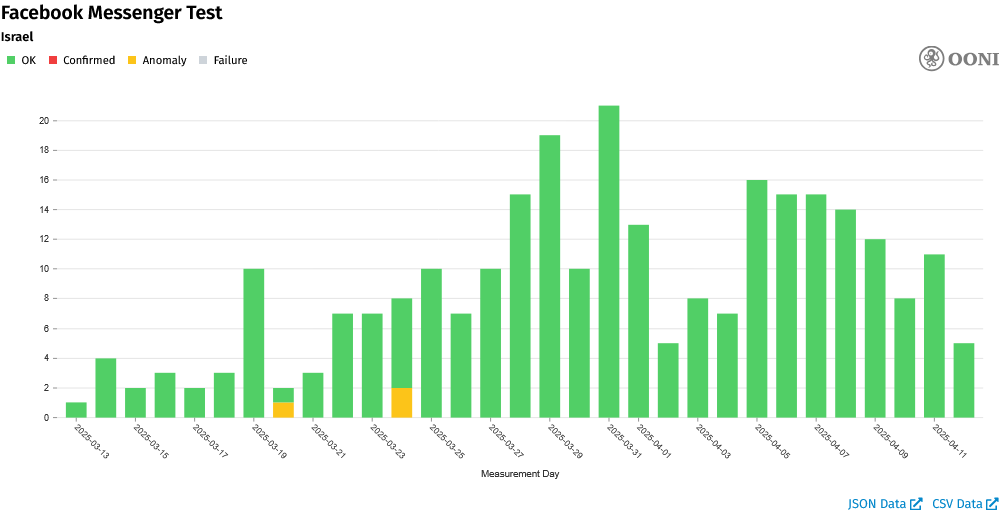
\includegraphics[width=0.5\linewidth]{ISROONIDBFB.png}
    \caption{Facebook Messenger test results for Israel 13/03-13/04}
    \label{fig:enter-label}
\end{figure}
\begin{figure} [H]
    \centering
    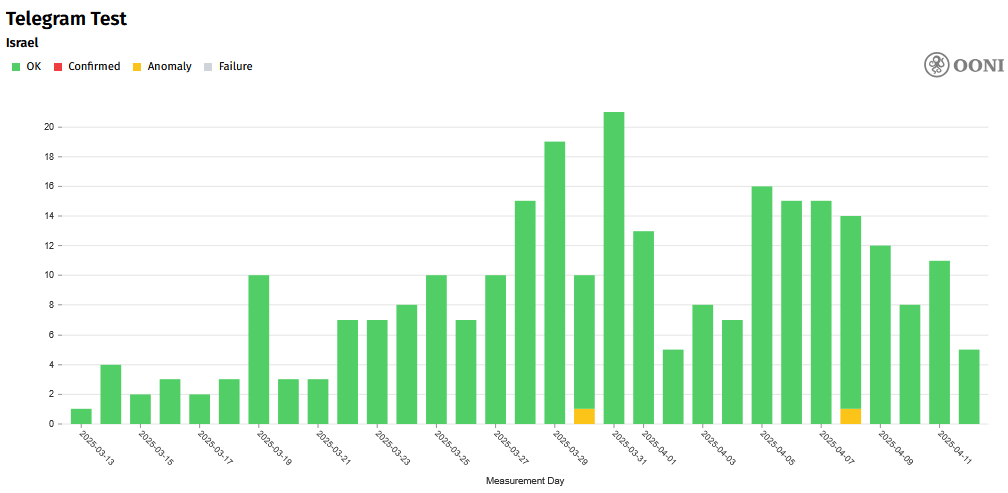
\includegraphics[width=0.5\linewidth]{ISROONIDBIM.png}
    \caption{Telegram test results for Israel 13/03-13/04}
    \label{fig:enter-label}
\end{figure}
\begin{figure} [H]
    \centering
    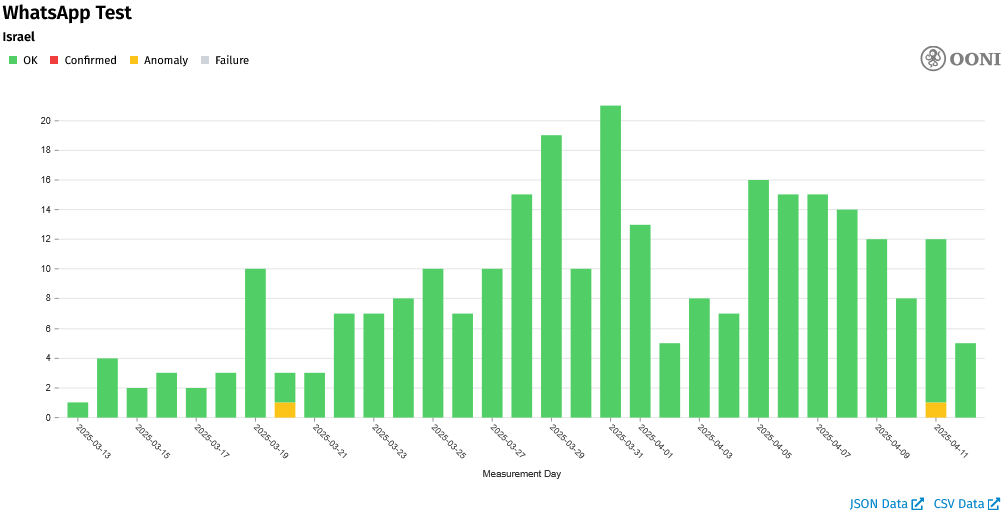
\includegraphics[width=0.5\linewidth]{ISROONIDBTEL.png}
    \caption{WhatsApp test results for Israel 13/03-13/04}
    \label{fig:enter-label}
\end{figure}
\begin{figure} [H]
    \centering
    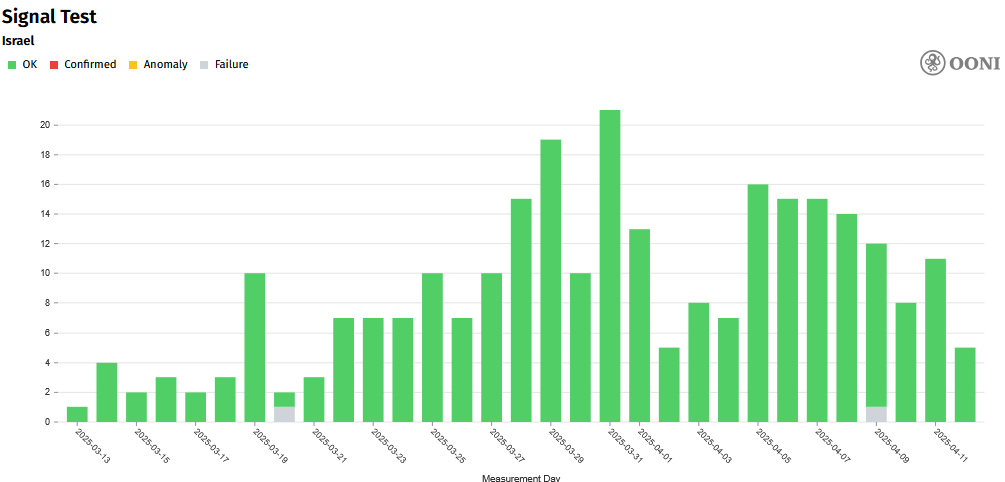
\includegraphics[width=0.5\linewidth]{ISROONIDBSIG.png}
    \caption{Signal test results for Israel 13/03-13/04}
    \label{fig:enter-label}
\end{figure}


\subsection{Ground Truth via SSH}
While running tests locally, no evidence for the blocking of instant messaging platforms was found in either Ireland or Israel. As seen in the above figures, there is little evidence in the OONI database to suggest either country interferes with instant messaging platforms. 


\section{Circumvention Tests}
\subsection{Public OONI Database: Ireland}

The majority of circumvention tests go unblocked in Ireland, however, certain ASNs show evidence of blocking. This can be see below.

\textbf{Ireland Circumvention Test Anomalies}
Based on data seen in the OONI database, TOR is not blocked by the majority of ASNs in Ireland. However, consistent blocking is seen in some networks. Over the period considered, there were seven instances of TOR being blocked, all attributed to HEAnet (AS 1213).

Psiphon appears to be blocked somewhat consistently on certain ASNs. The results are seen tabulated below, with a focus on ASNs containing anomalies.

\begin{table}[H]
\centering
\caption{Psiphon Circumvention Anomalies in Ireland}
\begin{tabular}{lccc}
\toprule
\textbf{Metric / ASN} & \textbf{Blocked} & \textbf{OK} & \textbf{\% Blocked} \\
\midrule
\textbf{Total}     & 82  & 575 & 12.48\% \\
\midrule
ASN 1213           & 57  & 6   & 90.48\% \\
ASN 6830           & 18  & 271 & 6.23\% \\
ASN 13280          & 5   & 13  & 27.78\% \\
ASN 9009           & 1   & 6   & 14.29\% \\
ASN 212238         & 1   & 0   & 100.00\% \\
ASN 8075           & 1   & 0   & 100.00\% \\
ASN 15751          & 1   & 8   & 11.11\% \\
\bottomrule
\end{tabular}
\label{tab:psiphon_ireland}
\end{table}



\begin{figure} [H]
    \centering
    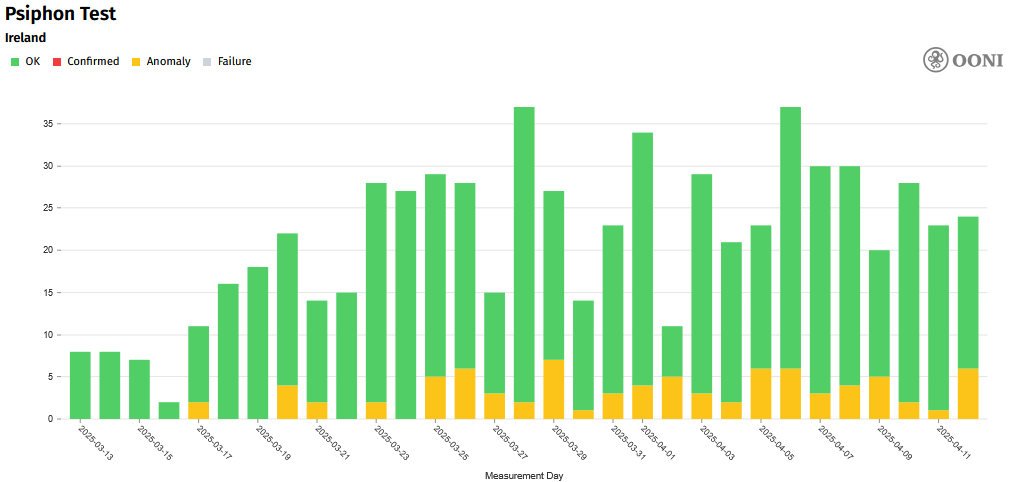
\includegraphics[width=0.5\linewidth]{IREDBPSI.png}
    \caption{Psiphon test results for Ireland 13/03-13/04}
    \label{fig:enter-label}
\end{figure}

\begin{figure} [H]
    \centering
    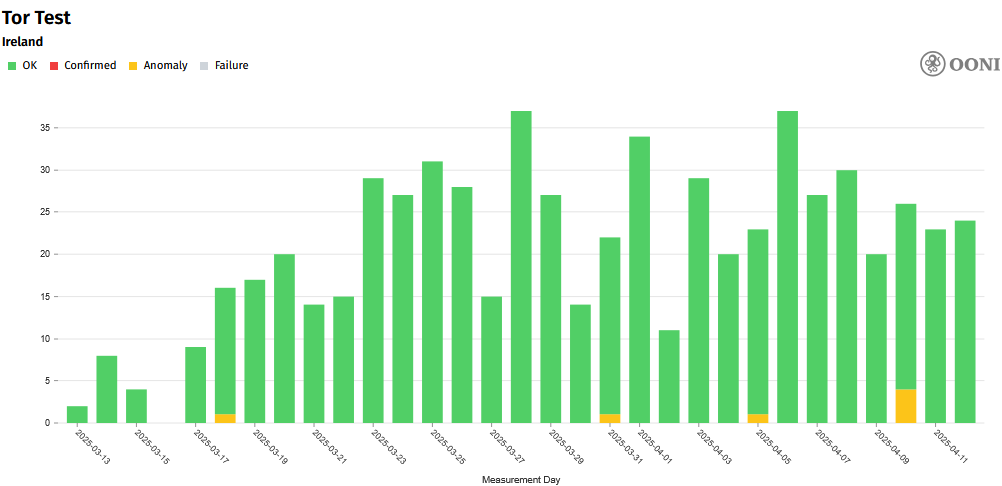
\includegraphics[width=0.5\linewidth]{IREDBTOR.png}
    \caption{TOR test results for Ireland 13/03-13/04}
    \label{fig:enter-label}
\end{figure}

\subsection{Public OONI Database: Israel}

Based on observations of the OONI database over the period of interest, TOR and Psiphon tests are not blocked in Israel. The only evidence of blocking comes from one autonomous system as described below.

\textbf{Israel Circumvention Test Anomalies}
ITC NG ltd (AS 202940) was responsible for 25 instances of blocking TOR connections and one instance of blocking Psiphon connections over the dates examined. This was the only ASN repsponsible for positive results. These anomalies are tabulated below.

\begin{table}[H]
\centering
\caption{Circumvention Results in Israel (ASN 202940)}
\begin{tabular}{lccc}
\toprule
\textbf{Tool} & \textbf{Blocked (Anomaly)} & \textbf{OK} & \textbf{\% Blocked} \\
\midrule
Psiphon & 1  & 27 & 3.57\% \\
Tor     & 25 & 3  & 89.29\% \\
\bottomrule
\end{tabular}
\label{tab:circumvention_israel}
\end{table}


\begin{figure} [H]
    \centering
    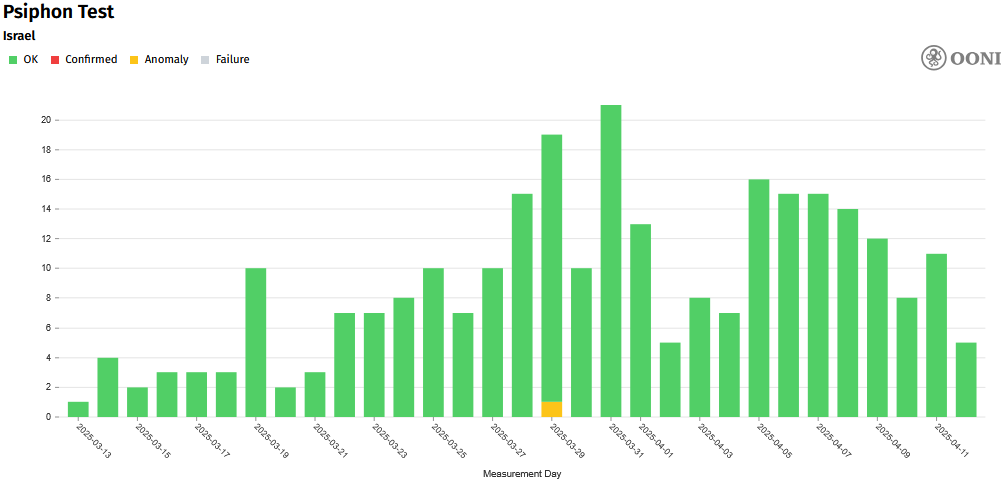
\includegraphics[width=0.5\linewidth]{ISROONIPSI.png}
    \caption{Psiphon test results for Israel 13/03-13/04}
    \label{fig:enter-label}
\end{figure}

\begin{figure} [H]
    \centering
    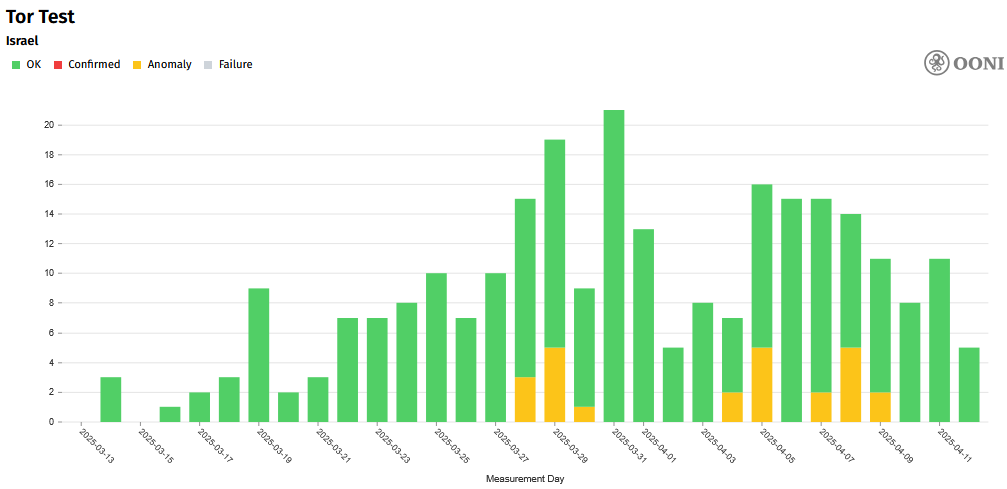
\includegraphics[width=0.5\linewidth]{ISROONITOR.png}
    \caption{TOR test results for Israel 13/03-13/04}
    \label{fig:enter-label}
\end{figure}

\subsection{Ground Truth via SSH}
No evidence for the blocking of TOR or Psiphon was found while running circumvention tests in either locale. This is consistent with the OONI database as in both countries, blocking appears inconsistent and AS specific.



\section{Middlebox Tests}
\subsection{Public OONI Database: Ireland}
In examining the OONI database for HTTP Invalid Request Line tests conducted in Ireland over the period of interest, only a handful of anomalies are observed. Out of the 660 HTTP Invalid Request Line tests conducted there were 5 anomalies. These instances belonged to M247 Europe SRL (AS9009), Vodafone Ireland Limited (AS15502) and Meteor Mobile Communications Limited (AS15751). A breakdown of the anomalies is seen below.

\begin{table}[H]
\centering
\caption{HTTP Invalid Request Line Test Anomalies in Ireland}
\begin{tabular}{lcc}
\toprule
\textbf{ASN} & \textbf{Anomalies} & \textbf{OK} \\
\midrule
\textbf{Total}   & 5 & 660 \\
\midrule
AS9009           & 3 & 4 \\
AS15502          & 1 & 103 \\
AS15751          & 1 & 9 \\
\bottomrule
\end{tabular}
\label{tab:http_invalid_ireland}
\end{table}



\begin{figure} [H]
    \centering
    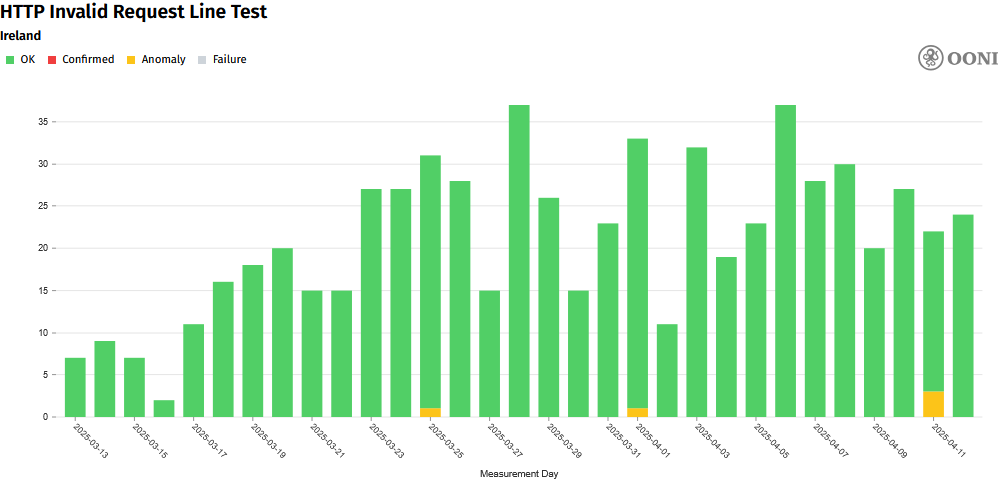
\includegraphics[width=0.5\linewidth]{IREOONIDBMB1.png}
    \caption{HTTP Invalid Request test results for Ireland 13/03-13/04}
    \label{fig:enter-label}
\end{figure}

Irish tests for HTTP Heaer Field Manipulation were less intriguing with only 6 anomalies over the period of interest. These were attributed to M247 Europe SRL (AS9009) and HEAnet (AS 1213) respectively. A breakdown of these results is seen below.


\begin{table}[H]
\centering
\caption{HTTP Header Field Manipulation Anomalies in Ireland}
\begin{tabular}{lccc}
\toprule
\textbf{ASN} & \textbf{Anomalies} & \textbf{OK} & \textbf{Percentage Anomalous} \\
\midrule
\textbf{Total}   & 6 & 648 & 0.91\% \\
\midrule
AS9009           & 2 & 1   & 66.67\% \\
AS1213           & 4 & 7   & 36.36\% \\
\bottomrule
\end{tabular}
\label{tab:http_header_ireland}
\end{table}

\begin{figure} [H]
    \centering
    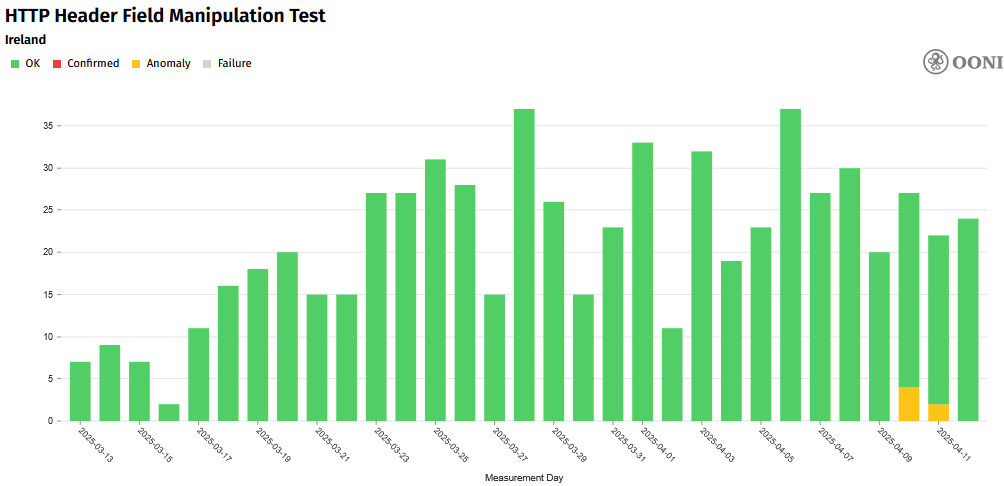
\includegraphics[width=0.5\linewidth]{IREOONIDBMB2.png}
    \caption{HTTP Header Field Manipulation test results for Ireland 13/03-13/04}
    \label{fig:enter-label}
\end{figure}







\subsection{Public OONI Database: Israel}
Only one instance of HTTP a Invalid Request Line anomaly was seen in Israel over the period of interest and belonged to XFone 018 Ltd (AS47956). 


\begin{figure} [H]
    \centering
    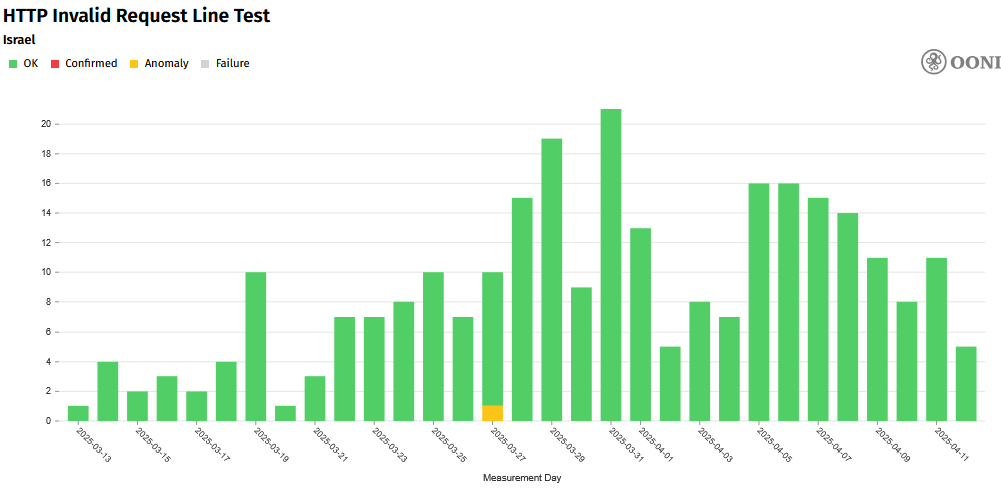
\includegraphics[width=0.5\linewidth]{ISROONIDBMB1.png}
    \caption{HTTP Invalid Request test results for Israel 13/03-13/04}
    \label{fig:enter-label}
\end{figure}

On the other hand, HTTP Header Field Manipulation test results for Israel were quite interesting. Anomalies were attributed to three different ASNs: Cellcom Fixed Line Communication L.P (AS1680), ITC NG ltd (AS202940) and XFone 018 Ltd (AS47956). The breakdown of these results is tabulated below.

\begin{table}[H]
\centering
\caption{HTTP Header Field Manipulation Anomalies in Israel}
\begin{tabular}{lccc}
\toprule
\textbf{ASN} & \textbf{Anomalies} & \textbf{OK} & \textbf{Percentage Anomalous} \\
\midrule
\textbf{Total}       & 35 & 237 & 12.87\% \\
\midrule
AS202940             & 25 & 4   & 86.21\% \\
AS1680               & 9  & 3   & 75.00\% \\
AS47956              & 1  & 7   & 12.50\% \\
\bottomrule
\end{tabular}
\label{tab:http_header_israel}
\end{table}


\begin{figure} [H]
    \centering
    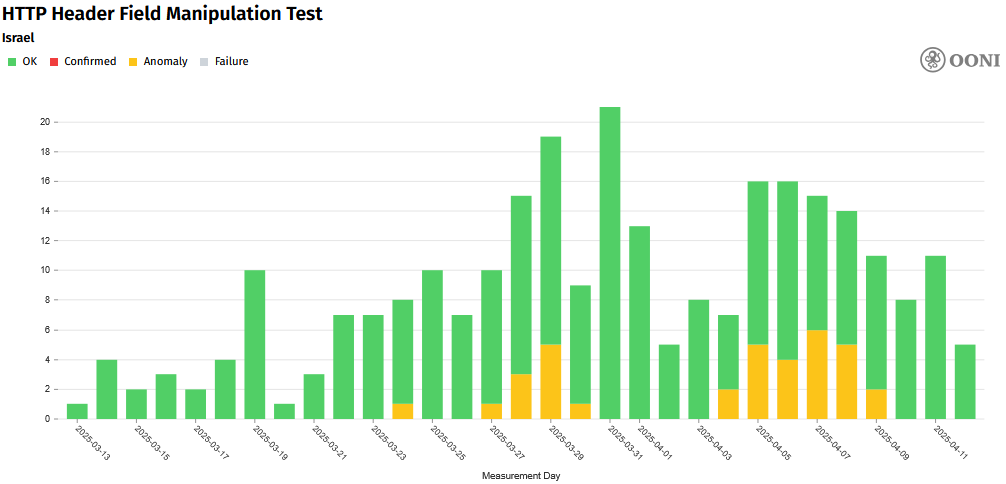
\includegraphics[width=0.5\linewidth]{ISROONIDBMB2.png}
    \caption{HTTP Header Field Manipulation test results for Israel 13/03-13/04}
    \label{fig:enter-label}
\end{figure}

\subsection{Ground Truth via SSH}
Results of running middlebox tests locally in both countries were uninteresting and no evidence of their presense was noted. However, as seen above Cellcom Fixed Line Communication L.P (AS1680) and ITC NG ltd (AS202940) are responsible for a significant number of positive with a majority of measurements showing interference. 



\section{Comparitive Analysis: Ireland vs. Israel}
\subsection{Summary: Irish Internet Censorship}
\subsection{Summary: Israeli Internet Censorship}
\subsection{}

\section{Guide to Replicating Results}

\subsection{Investigating Aljazeera.com}
Below are some commands I found helpful while investigating aljazeera.com.

\begin{figure} [H]
    \centering
    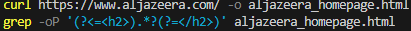
\includegraphics[width=1\linewidth]{AljazeeraURLs1.png}
    \caption{Using curl and grep to scrape URLs for articles}
    \label{fig:enter-label}
\end{figure}

\begin{figure} [H]
    \centering

\includegraphics[width=1\linewidth]{AljazeeraComs2.png}
    \caption{Inserting a dash after each URL, can now be ran with OONI}
    \label{fig:enter-label}
\end{figure}


\subsection{Raspberry Pi Setup}
\textbf{Operating System}
The operating system used was the latest available version of Raspberry Pi OS (64-bit) at the time of testing. It was flashed using the Raspberry Pi Imager application over USB. 

\begin{flushleft}
\hspace{1em}\textbf{Raspberry Pi OS (64-bit)}\\[0.5em]
\hspace{1em}Release date: November 19th 2024\\[0.5em]
\hspace{1em}System: 64-bit\\[0.5em]
\hspace{1em}Kernel version: 6.6\\[0.5em]
\hspace{1em}Debian version: 12 (bookworm)
\end{flushleft}


\textbf{Packages Installed}
In order to install the OONI probe CLI, the guide 'Install OONI Probe CLI on Debian/Ubuntu Linux' \cite{ooni-cli-install} was followed. The process was similar to that of installing on the Israeli VM. One obstacle faced in both instances were OpenPGP errors. To solve, the permissions for OONI probe had to be updated to bypass PGP signature verification. To do this, /etc/apt/sources.list.d/ooniprobe.list was edited to include '[trusted=yes]'

\begin{figure} [H]
    \centering
    
\includegraphics[width=0.75\linewidth]{PGPERROR.png}
    \caption{PGP Error installing CLI}
    \label{fig:enter-label}
\end{figure}



% unsrtnat
\bibliographystyle{abbrvnat}
\bibliography{bibs/sample}

\appendix
\renewcommand{\thechapter}{A\arabic{chapter}}
\chapter{Appendix}
You may use appendices to include relevant background information, such as calibration certificates, derivations of key equations or presentation of a particular data reduction method. You should not use the appendices to dump large amounts of additional results or data which are not properly discussed. If these results are really relevant, then they should appear in the main body of the report.

\section{Appendix numbering}
Appendices are numbered sequentially, A1, A2, A3\ldots The sections, figures and tables within appendices are numbered in the same way as in the main text. For example, the first figure in Appendix A1 would be Figure A1.1. Equations continue the numbering from the main text.

\section{Website Connectivity Tests: my-websites.txt}
\begin{multicols}{2}
\begin{itemize}
    \item \url{https://pbc.ps}
    \item \url{https://adultfriendfinder.com}
    \item \url{https://use-application-dns.net}
    \item \url{https://mgid.com}
    \item \url{https://exoclick.com}
    \item \url{https://rawa.org}
    \item \url{https://hamas.com}
    \item \url{https://coronavirus.app/}
    \item \url{https://chika.aangat.lahat.computer/}
    \item \url{https://censored.tv/}
    \item \url{https://outlook.live.com/}
    \item \url{http://kremlin.ru/}
    \item \url{https://kk.wikipedia.org/}
    \item \url{https://ru.wiktionary.org/}
    \item \url{https://ru.wikisource.org/}
    \item \url{https://pl.wikipedia.org/}
    \item \url{https://www.gov.ie/en/campaigns/c36c85-covid-19-coronavirus/}
    \item \url{https://ircz.de/}
    \item \url{https://thepiratebay.org/}
    \item \url{https://he.wikipedia.org/}
    \item \url{https://he.wikisource.org/}
    \item \url{https://he.wiktionary.org/}
    \item \url{http://www.phenoelit.org/}
    \item \url{https://www.pc2call.com/}
    \item \url{https://dnsleaktest.com/}
    \item \url{http://www.eurogrand.com/}
    \item \url{http://www.utorrent.com/}
    \item \url{http://www.socom.mil/}
    \item \url{https://www.rarbg.to/}
    \item \url{https://www.mp3.com/}
    \item \url{http://www.bittornado.com/}
    \item \url{http://www.bitcomet.com/}
    \item \url{https://thepiratebay.org/}
    \item \url{https://libgen.me/}
    \item \url{https://libgen.life/}
    \item \url{https://kickasstorrents.to/}
    \item \url{https://kat.am/}
    \item \url{http://www.oic-oci.org/}
    \item \url{http://www.islamdoor.com/}
    \item \url{https://www.iconnecthere.com/}
    \item \url{https://www.bittorrent.com/}

    \item \url{https://app.simplelogin.io/}
    \item \url{http://abpr2.railfan.net/}
    \item \url{https://www.xroxy.com/}
    \item \url{https://www.secfirst.org/}
    \item \url{http://www.queernet.org/}
    \item \url{https://secfirst.org/}
    \item \url{https://1.1.1.1/}
    \item \url{https://www.gamku.com/}
    \item \url{https://www.onlinearabiccasino.com/}
    \item \url{http://www.absinth.com/}
    \item \url{https://www.literotica.com/}
    \item \url{https://www.iasj.net/}
    \item \url{https://nazarene.org/}
    \item \url{http://www.on-instant.com/}
    \item \url{http://www.mailinator.com/}
    \item \url{http://www.euthanasia.cc/}
    \item \url{http://www.blogeasy.com/}
    \item \url{http://alhikmae.com/}
    \item \url{https://www.jsf.mil/}
    \item \url{https://www.rte.ie/}
    \item \url{https://www.chatgpt.com/}
    \item \url{https://www.independent.ie/}
    \item \url{https://www.dailymail.co.uk/}
    \item \url{https://www.bbc.com/}
    \item \url{https://www.donedeal.ie/}
    \item \url{https://www.yahoo.com/}
    \item \url{https://www.daft.ie/}
    \item \url{https://www.rip.ie/}
    \item \url{https://www.irishtimes.com/}
    \item \url{https://www.tiktok.com/}
    \item \url{https://www.irishexaminer.com/}
    \item \url{https://www.theguardian.com/}
    \item \url{https://www.aib.ie/}
    \item \url{https://www.sky.com/}
    \item \url{https://www.thejournal.ie/}
    \item \url{https://www.news.sky.com/}
    \item \url{https://www.nytimes.com/}
    \item \url{https://www.thesun.ie/}
    \item \url{https://www.met.ie/}
    \item \url{https://www.skysports.com/}
    \item \url{https://www.dublinlive.ie/}
    \item \url{https://www.boards.ie/}
    \item \url{https://www.bbc.co.uk/}
    \item \url{https://www.irishmirror.ie/}
    \item \url{https://www.xvideos.com/}
    \item \url{https://www.imdb.com/}
    \item \url{https://www.breakingnews.ie/}
    \item \url{https://www.galwaybeo.ie/}
    \item \url{https://www.lekmanga.net/}
    \item \url{https://www.shabakaty.com/}
    \item \url{https://www.kurdcinama.com/}
    \item \url{https://www.xhamster.com/}
    \item \url{https://www.reddit.com/}
    \item \url{https://www.xnxx.com/}
    \item \url{https://www.kurdsubtitle.net/}
    \item \url{https://www.like-manga.net/}
    \item \url{https://www.topcinema.cam/}
    \item \url{https://www.telegram.org/}
    \item \url{https://www.egydead.fyi/}
    \item \url{https://www.arabshentai.com/}
    \item \url{https://www.uptodown.com/}
    \item \url{https://www.beenar.net/}
    \item \url{https://www.xnxx-arabic.com/}
    \item \url{https://www.witanime.cyou/}
    \item \url{https://www.dailymotion.com/}
    \item \url{https://www.lodynet.io/}
    \item \url{https://www.weather.com/}
    \item \url{https://www.hentaislayer.net/}
    \item \url{https://www.live.com/}
    \item \url{https://www.xhexperience.xyz/}
    \item \url{https://www.theporndude.com/}
    \item \url{https://www.xvideos-ar.com/}
    \item \url{https://www.azoramoon.com/}
    \item \url{https://www.kisskh.co/}
    \item \url{https://www.kurdfilm.krd/}
    \item \url{https://www.arabx.cam/}
    \item \url{https://www.sexalarab.com/}
    \item \url{https://www.netflix.com/}
    \item \url{https://www.discord.com/}
    \item \url{https://www.twitch.tv/}
    \item \url{https://www.chess.com/}
    \item \url{https://www.tumblr.com/}
    \item \url{https://www.deviantart.com/}
    \item \url{https://www.wattpad.com/}
    \item \url{https://www.omegle.com/}
    \item \url{https://www.lichess.org/}
    \item \url{https://www.spankbang.com/}
    \item \url{https://www.bilibili.com/}
    \item \url{https://www.redtube.com/}
    \item \url{https://www.9gag.com/}
    \item \url{https://www.onlyfans.com/}
    \item \url{https://www.fanfiction.net/}
    \item \url{https://www.artstation.com/}
    \item \url{https://www.furaffinity.net/}
    \item \url{https://www.poki.com/}
    \item \url{https://www.vk.com/}
    \item \url{https://www.creepypasta.com/}
    \item \url{https://www.zoro.to/}
    \item \url{https://www.youporn.com/}
    \item \url{https://www.etsy.com/}
    \item \url{https://www.vimeo.com/}
    \item \url{https://www.pixiv.net/}
    \item \url{https://www.rule34.xxx/}
    \item \url{https://www.redgifs.com/}
    \item \url{https://www.stripchat.com/}
    \item \url{https://www.opera.com/}
    \item \url{https://www.wikipedia.com/}
    \item \url{https://www.foxnews.com/}
    \item \url{https://www.porn.com/}
    \item \url{https://www.russia.tv/}
    \item \url{https://www.rt.com/}
    \item \url{https://www.beeg.com/}
    \item \url{https://www.4chan.org/}
    \item \url{https://www.crunchyroll.com/}
    \item \url{https://www.mozilla.org/}
\end{itemize}
\end{multicols}


\section{sample\_aljazeeraurls.txt}
\begin{itemize}
    \item \url{https://www.aljazeera.com/news/liveblog/2022/10/16/ukraine-russia-live-news-russian-forces-repel-ukraine-advances/}
    \item \url{https://www.aljazeera.com/economy/2023/10/27/shifting-politics-make-india-a-hotbed-for-israel-hamas-war-misinformation/}
    \item \url{https://www.aljazeera.com/economy/2022/10/10/what-a-us-recession-would-mean-for-the-world/}
    \item \url{https://www.aljazeera.com/economy/2021/10/11/energy-crunch-qatar-says-lng-production-maxed-out/}
    \item \url{https://www.aljazeera.com/economy/2006/12/15/made-in-china-worrying-the-us/}
    \item \url{https://www.aljazeera.com/economy/2009/10/14/video-russian-pensioners-struggle/}
    \item \url{https://www.aljazeera.com/economy/2009/10/20/video-lebanon-firms-invest-in-iraq/}
    \item \url{https://www.aljazeera.com/economy/2014/10/12/israeli-blockade-cripples-gazas-economy/}
    \item \url{https://www.aljazeera.com/economy/2024/10/10/td-bank-pleads-guilty-to-us-charges-faces-business-restrictions/}
    \item \url{https://www.aljazeera.com/economy/2024/10/11/boeing-to-cut-10-workforce-delay-777x-delivery-as-strike-takes-toll/}
    \item \url{https://www.aljazeera.com/economy/2024/10/11/indias-ratan-tata-the-man-who-knew-how-to-think-big-and-bold/}
    \item \url{https://www.aljazeera.com/economy/2024/10/11/indonesia-eyes-hefty-tariffs-on-china-as-businesses-decry-cheap-imports/}
    \item \url{https://www.aljazeera.com/economy/2024/10/11/taiwan-says-four-employees-of-apple-supplier-foxconn-arrested-in-china/}
    \item \url{https://www.aljazeera.com/economy/2024/10/11/teslas-robotaxi-event-was-long-on-musk-promises-short-on-details/}
    \item \url{https://www.aljazeera.com/economy/2024/10/14/acting-us-labour-secretary-to-meet-with-boeing-and-union-to-end-impasse/}
    \item \url{https://www.aljazeera.com/economy/2024/10/14/poorest-countries-in-worst-financial-shape-since-two-thousand-six-world-bank-says/}
    \item \url{https://www.aljazeera.com/economy/2024/10/15/air-taxi-growth-demands-efficient-vertiports-and-traffic-control-systems/}
    \item \url{https://www.aljazeera.com/gallery/liveblog/2024/6/4/israels-war-on-gaza-live-pressure-mounts-on-israel-hamas-to-cease-fire/}
    \item \url{https://www.aljazeera.com/news/liveblog/2022/10/10/several-explosions-heard-in-ukraine-capital-kyiv/}
    \item \url{https://www.aljazeera.com/news/liveblog/2022/10/11/russia-ukraine-live-news-more-strikes-hit-zaporizhzhia/}
    \item \url{https://www.aljazeera.com/news/liveblog/2022/10/12/russia-ukraine-live-news-biden-doubts-use-of-nuclear-weapons/}
    \item \url{https://www.aljazeera.com/news/liveblog/2022/10/13/jan-6-panel-live-news-us-committee-holds-9th-public-hearing/}
    \item \url{https://www.aljazeera.com/news/liveblog/2022/10/13/ukraine-russia-live-news-kyiv-area-hit-by-kamikaze/}
    \item \url{https://www.aljazeera.com/news/liveblog/2022/10/14/russia-ukraine-live-news-ukraine-retook-75-kherson-settlements/}
    \item \url{https://www.aljazeera.com/news/liveblog/2022/10/15/russia-ukraine-live-news-shelling-fire-at-russian-fuel-depot/}
    \item \url{https://www.aljazeera.com/news/liveblog/2022/10/16/la-liga-real-madrid-vs-barcelona-as-it-happened/}
    \item \url{https://www.aljazeera.com/economy/longform/2022/12/22/the-protests-that-exposed-cracks-in-chinas-middle-class-dream/}
    \item \url{https://www.aljazeera.com/economy/longform/2023/11/24/a-fire-two-deaths-and-the-business-of-elder-care-in-india/}
    \item \url{https://www.aljazeera.com/economy/longform/2023/7/12/sri-lankas-fishermen-face-double-whammy-of-climate-and-economy-3/}
    \item \url{https://www.aljazeera.com/economy/longform/2024/4/20/when-will-our-good-days-come-the-mumbai-cook-voting-in-indias-elections/}
    \item \url{https://www.aljazeera.com/economy/longform/2024/4/24/parallel-economy-how-russia-is-defying-the-wests-boycott/}
    \item \url{https://www.aljazeera.com/economy/longform/2024/5/2/after-years-of-decline-a-new-generation-of-organised-labour-rises-in-us/}
    \item \url{https://www.aljazeera.com/economy/longform/2024/6/11/the-future-is-dark-inside-the-brazilian-businesses-shattered-by-floods/}
    \item \url{https://www.aljazeera.com/features/longform/2021/11/16/snatched-away-the-indigenous-women-taken-on-the-highway-of-tears/}
    \item \url{https://www.aljazeera.com/features/longform/2021/11/19/after-cop26-letdown-can-indias-gen-z-climate-warriors-prevail/}
    \item \url{https://www.aljazeera.com/features/longform/2021/11/29/hunted-how-indigenous-women-are-disappearing-in-canada/}
\end{itemize}


\end{document}